\documentclass[12pt]{book}
\usepackage{booktabs}
\usepackage[table]{xcolor}
\usepackage{tcolorbox}
\usepackage[T1]{fontenc}
\usepackage{wrapfig}
\usepackage{url}
\usepackage{dsfont}
\usepackage{enumitem}
\usepackage{array}
\usepackage{booktabs}
\usepackage{multirow}
\usepackage{mathtools, nccmath}
\usepackage[polish]{babel}
\usepackage[utf8]{inputenc}
\usepackage{lmodern}
\usepackage{pifont}
\usepackage{blkarray, bigstrut}
\usepackage{amsmath}
\usepackage{kbordermatrix}
\usepackage{cases}
\usepackage{graphicx}
\usepackage{cellspace}
\usepackage[T1]{fontenc}
\usepackage{amsthm}
\selectlanguage{polish}
\usepackage{amsmath}
\usepackage{graphicx}
\usepackage{float}
\usepackage{cite}
\usepackage[margin=2.5cm]{geometry}
\theoremstyle{plain}
\newtheorem{definicja}{Definicja}
\newtheorem{twr}{Twierdzenie}
\newtheorem{lem}[twr]{Lemat}
\newtheorem{mur}{Murphy}[section]
\newcolumntype{P}[1]{>{\centering\arraybackslash}p{#1}}
\newcommand\green{\cellcolor{green!10}}
\newcommand\cincludegraphics[2][]{\raisebox{-0.5\height}{\includegraphics[#1]{#2}}}
\newcommand\red{\cellcolor{red!20}}
\newcommand\blue{\cellcolor{blue!20}}
\newcommand{\R}{\mathbb{R}}
\newcommand*{\tabbox}[2][t]{%
	\vspace{0pt}\parbox[#1][3.7\baselineskip]{1cm}{\strut#2\strut}}
\newcommand\addtag{\refstepcounter{equation}
\renewcommand{\labelenumii}{\theenumii}
\renewcommand{\theenumii}{\theenumi.\arabic{enumii}.}
\tag{\theequation}}
\newcommand{\myref}[1]{(\ref{#1})} 
\newcommand{\specialcell}[2][c]{%
	\begin{tabular}[#1]{@{}c@{}}#2\end{tabular}}

\begin{document}
\title{Optymalizacja  systemu sygnalizacji świetlnej w 
oparciu o przepływowy model ruchu pojazdów.}
\author{Michał Lis}
\date{\today}
\maketitle
\tableofcontents
\chapter{Wprowadzenie}
Problem zatłoczonych ulic staje się coraz bardziej powszechny na całym świecie. W ostatnich latach obserwowany jest ogromny wzrost ilość pojazdów na drogach.
%Problem zatłoczonych ulic staje się coraz bardziej powszechny na całym świecie, głównie ze względu na wzrost ekonomiczny. Według banku światowego w roku 1990 suma produktów krajowych brutto wszystkich państw świata wynosiła 22,6 biliona dolarów \cite{worldBank}. Najbardziej aktualne dane banku światowego dotyczą lat 2012-2017. W czasie ich trwania analogiczna wartość oscylowała wokół 75 bilionów dolarów. Nawet przy uwzględnieniu inflacji dolara, która od w okresie 1990 do 2015 wyniosła $80\%$ światowy produkt brutto jest obecnie prawie dwukrotnie większy w porównaniu do roku 1990. Bezpośrednim skutkiem ogólnoświatowego wzrostu stopy życiowej jest zwiększenie ilości samochodów na drogach.
Według danych statystycznych firmy \textit{Statista} liczba zarejestrowanych pojazdów na świecie w roku 2006 wynosiła 947 tysięcy \cite{liczbaPojazdowSwiat}. W 2015 roku na świecie jeździło już 1282 tysięcy pojazdów. Wzrost przez te 9 lat był niemalże liniowy. Co roku rejestrowano około 40 tysięcy nowych samochodów rocznie, co wyznacza stopę wzrostu liczby pojazdów na poziomie 3,7$\%$ w skali roku.
\begin{figure}[H]
  \centering
    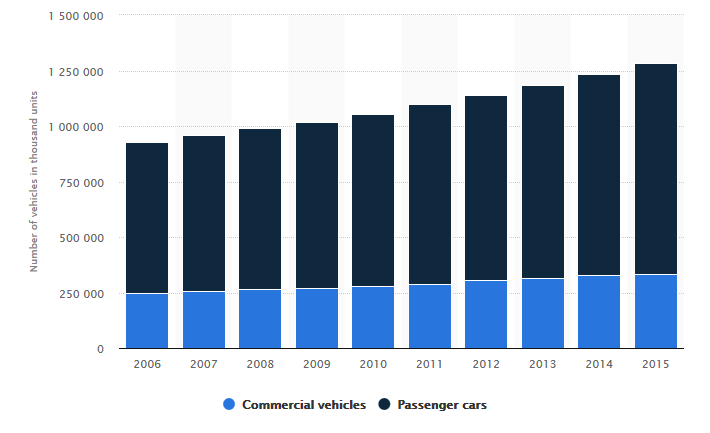
\includegraphics[width=14cm]{liczbaPojazdowSwiat}
 \caption{Liczba pojazdów na świecie}
 \label{fig:liczbaPojazdowSwiat}
\end{figure} \noindent
W Polsce wzrost ilości pojazdów w latach 2006 - 2015 był jeszcze większy \cite{liczbaPojazdowPolska}. W 2006 roku według GUS w Polsce było zarejestrowanych 13,4 miliona samochodów osobowych. W 2015 roku ich liczba wynosiła już 20,7 miliona, co wyznacza 5 procentowy roczny wzrost ilości pojazdów.
Najbardziej zatłoczonym polskim miastem jest Łódź. Według rankingu firmy \textit{TomTom } Łódź zajmuje bardzo wysokie 5 miejsce na świecie i 1 w Europie pod względem zatłoczenia dróg \cite{rankingTomTom}. Oprócz Łodzi w pierwszej setce najbardziej zatłoczonych miast świata są inne polskie miasta: Lublin(34), Kraków(48), Warszawa(50), Wrocław(63), Poznań(69), Bydgoszcz(83). Zatory drogowe są jednak problem całej Europy. Spośród 100 najbardziej zatłoczonych miast świata aż 45 znajduje się w Europie. W 2008 roku Unia Europejska oszacowała, iż koszty zatłoczenia dróg kształtują się na poziomie $0,9\%-1,5\%$ PKB unijnego \cite{ue2008}. Następny raport z 2017 roku może napawać optymizmem, gdyż przedstawione w nim wyliczenia określiły jedynie $0,77\%$ straty całkowitego PKB wspólnoty \cite{ue2017}. Ten sam raport ocenia koszty zatorów komunikacyjnych w Polsce na poziomie $1,2\%$ polskiego PKB.
Problemy zatorów komunikacyjnych w miastach są o tyle trudniejsze do rozwiązania niż poza miastem, ponieważ na terenach zurbanizowanych często brakuje miejsca na wybudowanie dróg o większej przepustowości. Rozwiązaniem może być wprowadzenie większej ilości sygnalizacji świetlnych. Istotną kwestią jest optymalizacja ustawień sygnalizacji świetlnej. Praca jest poświęcona przede wszystkim temu aspektowi. Zostaną w niej także przedstawione matematyczne modele sieci drogowej oraz ich komputerowe symulacje. 
%W celu uzyskania danych potrzebnych do tego procesu rozstawiane są na drogach detektory ruchu. 
%\begin{figure}[H]
%  \centering
%    \includegraphics[width=14cm]{Detektor}
% \caption{System pętli do detekcji osi pojazdów zainstalowany na badawczym stanowisku pomiarowym na drodze DK81 będący w dyspozycji Katedry Metrologii i Elektroniki AGH.}
% \label{fig:Detektor}
%\end{figure} \noindent
%W miastach zachodnioeuropejskich rezultaty naprawdę widać dopiero po roku, gdy system zgromadzi już ogromną ilość danych - mówi Misiorny
%
%Czytaj więcej: https://dzienniklodzki.pl/masz-uwagi-do-sygnalizacji-swietlnej-w-lodzi-wyslij-email-do-zdit/ar/9253440
\chapter{Cel i zakres pracy}
W rozdziale \ref{chapter:model_sieci_drog} przedstawiony zostanie model sieci dróg. Stworzony przez autora pracy został program symulujący ruch drogowy. Jest on napisany w języku Python (wersja 3.6). Oddzielna warstwa wizualizacyjna utworzona w typescriptowym frameworku Angular w wersji 6. Grafiki przedstawiające środowiska drogowe są narysowane przy pomocy tagów canvas. Kroki potrzebne do uruchomienia programu zostały przedstawione w TODO rozdział do napisania na sam koniec.
Bezpośrednim celem pracy jest uzyskanie płynnego ruchu przy możliwie dużej ilości pojazdów wjeżdżających do rozważanego środowiska. Ostatnie środowisko testowe w pracy przedstawia sieć dróg wokół kampusu B Politechniki Łódzkiej i to głównie na optymalizacji tego środowiska będzie skupiona uwaga. Wszystkie poprzednie sieci dróg są mniej skomplikowane i służą głównie przy przedstawieniu modelu i procesu optymalizacji.
Środowiska będą skonstruowane w pełni zgodne z makroskopowym modelem ruchu, który nie rozróżnia indywidualnych pojazdów, a traktuje je jako ilościowo. Sam makroskopowy model ruchu zostanie przedstawiony w rozdziale \ref{chapter:makroskopowy_model_ruchu}. Początkowy model będzie bardzo prosty z pominięciem większości aspektów. W każdej kolejnej sekcji model będzie stopniowo rozwijany.

\chapter{Makroskopowy model ruchu} \label{chapter:makroskopowy_model_ruchu}
\section{Klasyfikacja modeli ruchu drogowego}
Modele ruchu drogowego mają na celu ukazanie rzeczywistego przepływu pojazdów w sposób czysto matematyczny. Ważnym kryterium doboru modelu jest przystępność jego implementacji informatycznej. Powszechnie klasyfikuje się 3 podejścia modelowe dla omawianego problemu \cite{CompareModels} - makroskopowy, mezoskopowy oraz mikroskopowy. Czasem \cite{multilevel} wyróżnia się także czwarte podejście - submikroskopowe. Jest to podział ze względu na poziom modelu. Najniższy poziom i najbardziej dokładny model gwarantuje podejście mikroskopowe. Rozważa ono pojazdy indywidualnie w czasoprzestrzeni. Przyspieszenie pojazdu jest wyliczane na podstawie dynamiki(prędkości, przyspieszenia) i pozycji pojazdu bezpośrednio przed nim. Model mezoskopowy zapewnia indywidualne rozróżnienie pojazdów, jednak ich zachowanie jest wyliczane na danych zagregowanych \cite{mesoscopic}. Przykładowo pojazdy są podzielone na grupy podróżujące od pewnego punktu startowego do punktu końcowego. Inne modele \cite{mesoscopic2} mezoskopowe wyliczają dynamikę ruchu na podstawie aktualnego zatłoczenia drogi. Poziom mezoskopowy jest obliczeniowo bardziej opłacalny od mikroskopowego.
Wiele symulatorów stosujących model mezoskopowy oferuje symulację w czasie rzeczywistym dla sieci dróg całego miasta\cite{vu2017high}. Ideą modelu makroskopowego jest traktowanie ruchu ulicznego identycznie jak ruchu cieczy lub gazów. Po raz pierwszy w roku 1956 M. J. Lighthill i G. B. Whitham \cite{lwr} przedstawili pomysł przyrównania ruchu ulicznego na zatłoczonych drogach do przepływu wody w rzekach. Z tego powodu nie uznajemy w nim pojazdów jako niepodzielne jednostki. Pojazd można przyrównać do pewnej ilości wody w rzece.
Jest to najmniej kosztowny obliczeniowo model. Właśnie w modelu makroskopowym zostało stworzone środowisko symulacyjne. Szczegóły modelu są przedstawione w następnym podrozdziale.

\section{Wstęp}
Jako zmienną stanową makroskopowego modelu ruchu zazwyczaj wybierana jest gęstość ruchu \cite{gottlich,CompareModels}. Formalnie gęstość można rozumieć jako czynnik definiujący dynamikę ruchu. Im większa jest gęstość tym mniejsza prędkość ruchu. Gęstość ruchu \cite{helbing2001master} jest przedstawiona jako iloraz ilości pojazdów znajdujących się na pewnym odcinku i długości tego odcinka drogi. Prawidłowe jest także uznanie ilości pojazdów na pojedynczym odcinku drogi jako zmienną stanową. Należy jednak pamiętać, że pojazdy w ruchu makroskopowym nie są nierozłączną jednostką. Pojazd w analogii do przepływu wody w rzece jest pewną jednostką wody. Wielokrotnie w symulacjach zdarza się, że na odcinku jest zatem niecałkowita liczba pojazdów.

\section{Rozwój gęstości ruchu na drodze}
Makroskopowy model ruchu jest oparty o równanie różniczkowe (\ref{eq:main_diff_eq}) wraz z warunkiem początkowym (\ref{eq:p_init_eq}) \cite{gottlich}. W analogii do przepływu wody w rzece gęstość ruchu można utożsamiać z polem powierzchni przekroju poprzecznego rzeki, co dla stałej szerokości rzeki - upraszcza się do wysokości wody w rzece.   \\Dla ustalonej pojedynczej drogi zmianę gęstości ruchu definiuje następujący układ równań:\\
\begin{numcases}{}
   p(x,0)=p_{0}(x) \label{eq:p_init_eq}
   \\
   \frac{\partial p(x,t)}{\partial t}+\frac{\partial f(p(x,t))}{\partial x}=0 \label{eq:main_diff_eq}
\end{numcases}
Gdzie $p(x,t)$ to gęstość ruchu w punkcie $x$ i czasie $t$. Wartość funkcji gęstości należy do przedziału $[0,p^{max}]$.\\
Równanie (\ref{eq:p_init_eq}) zakłada istnienie pewnej z góry nałożonej początkowej gęstości drogi $p_0(x)$.
Równianie (\ref{eq:main_diff_eq}) określa
wedle założeń modelu makroskopowego \cite{lwr} rozwój gęstości ruchu na drodze. Funkcja płynności ruchu $f$ powinna być wklęsła \cite{gottlich}. 
%W przedstawionym w tej pracy modelu funkcja ma następującą definicję:
%\begin{numcases}{f(p)=}
%   \lambda p & \text{dla } $p\in[0,p^{*}]$\\
%   \lambda \cdot (2p^{*}-p) & \text{dla } $p\in(p^{*},p^{max}]$ 
%\end{numcases}
%Gdzie $\lambda$ jest stałym parametrem funkcji trójkątnej oraz $p^*=\frac{1}{2}p^{max}$.
\section{CTM - Cell Transmission Model}
\subsection{Wprowadzenie}
W tym rozdziale zostanie przedstawiony model CTM będący dyskretyzacją pierwotnego modelu makroskopowego przepływu \cite{lwr}. Jego zmienną stanową jest ilość pojazdów. Model został opisany w artykule Carslosa Daganzo \cite{CTM} w 1992. Ta pozycja jest podstawą wszelkich wyliczeń w tym rozdziale.
\subsection{Przedstawienie modelu}
\subsection*{Siatka czasowa i przestrzenna drogi}
Dyskretny charakter modelu CTM obliguje do określenia siatki czasowej i przestrzennej drogi. Dla par czasu i miejsc należących do tych dwóch siatek będą określane zmienne stanu. \\ \\ \textbf{Siatka czasowa} jest zdefiniowana jako skończony ciąg liczb naturalnych:
\[(0,1,...,T). \addtag \]
Następnie zdefiniowana zostanie siatka przestrzenna drogi e. Ustalona droga e to odcinek $[0,L]$. Zostaje ona podzielona na $L$ odcinków o równej długości. \textbf{Siatka przestrzenna} drogi to ciąg odcinków:
\[([0,1),[1,2),...,[L-1,L] )\]

\subsection*{Przepływ pojazdów na drodze}
Niech dana będzie droga $e$ i pewien odcinek $i$ na tej drodze. Zmienna stanowa w modelu CMT jest oznaczana jako $n_i(t)$ i określa ona ilość pojazdów na odcinku $i$ w chwili t.
Przepływ pojazdów opiera się o założeniu, iż przy braku zatorów pojazdy pokonują w jednym interwale czasowym jeden odcinek drogi. Przykładowy przepływ jest następujący:
\begin{figure}[H]
	\centering
	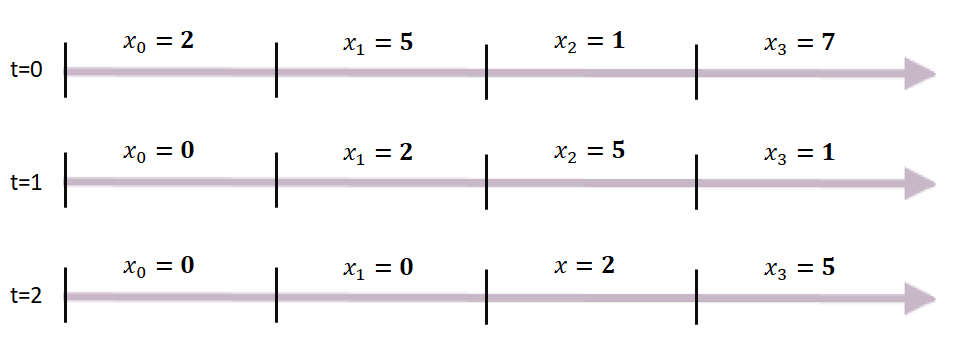
\includegraphics[width=14cm]{images/CTM_flow_example}
	\caption{Przykładowy przepływ bez zatorów w modelu CTM}
	\label{fig:CTM_flow_example}
\end{figure} \noindent
Łatwo zauważyć, że w tym przypadku
\[ n_{i+1}(t+1)=n_i(t) \addtag \]
\subsubsection*{Wprowadzenie zatorów}
W celu wprowadzenia pojęcia zatoru zostaną zdefiniowane następujące zmienne:

\begin{itemize}
	\item $N_i(t)$ - maksymalna ilość pojazdów, które mogą znajdować się na odcinku $i$ w chwili $t$.
	\item $Q_i(t)$ - maksymalna ilość pojazdów, które mogą napłynąć do odcinka $i$ w momencie $t+1$.
\end{itemize}
Rozwój zmiennej stanowej jest zadany poprzez następujące równanie:
\[n_i(t+1)=n_i(t)+y_i(t)-y_{i+1}(t) \addtag \]
Gdzie:
\begin{itemize}
	\item $y_i(t)$ to ilość pojazdów napływających do odcinka $i$ w chwili $t+1$.
	\item $y_{i+1}(t)$ to ilość pojazdów napływających do odcinka $i+1$ w chwili $t+1$. Jest to zatem także ilość pojazdów opuszczających odcinek $i$ w interwale $[t,t+1)$.
\end{itemize}
Przepływ pojazdów $y_i(t)$ jest zdefiniowany jako minimum z następujących trzech wartości:
\begin{itemize}
	\item $ n_{i-1}(t) $ - ilość pojazdów na poprzedzającym odcinku (t.j. $i-1$)
	\item $ Q_i(t) $ - maksymalna ilość pojazdów, które mogą napłynąć do odcinka $i$ w chwili $t+1$.
	\item $ N_i(t)-n_i(t) $ - ilość wolnych miejsc na odcinku $i$ w chwili $t$
\end{itemize}
Co wyraża się wzorem:
\[
y_i(t)=Min\{n_{i-1}(t),Q_i(t),N_i(t)-n_i(t)\} \addtag \label{eq_y_CTM}
\]
\subsection*{Źródło i ujście ruchu}
Powyższe wzory potrzebują ustaleń odnośnie źródła i ujścia ruchu. Bez nich wzór \myref{eq_y_CTM} nie ma sensu dla krańcowych odcinków $i=0$ oraz $i=L$. Dla ułatwienia pogrubione zostały ustalone w tym rozdziale wartości zmiennych źródła i ujścia ruchu. \\ Źródło ruchu może być traktowane jako odcinek o indeksie $i=-1$. Jedyną wartością, która musi być ustalona dla źródła jest ilość pojazdów w nim, czyli $n_{i-1}(t)$. Przyjęte zostaje, że $\mathbf{n_{i-1}(t)=\infty}$ - wtedy napływ pojazdów do odcinka $i=0$ jest ograniczony z dołu już tylko przez $Q_0(t)$ oraz $N_0(t)-n_0(t)$.
\\
Ujście ruchu z kolei może być traktowane jako odcinek $i=L+1$. Istotne w kontekście wzoru \myref{eq_y_CTM} są następujące wartości:
\begin{itemize}
	\item $Q_{L+1}(t)$ - ilość pojazdów, które mogą opuścić odcinek $L$ w chwili $t$. Ustalone jest, że jest to dowolna ilość, wtedy $\mathbf{Q_{L+1}(t)=\infty}$
	\item $N_{L+1}(t)$ - ilość pojazdów, które może pomieścić ujście. Ustalone jest, że $\mathbf{N_{i}(t)=\infty}$, gdyż ujście może zawierać nieograniczoną ilość pojazdów.
	\item $n_{L+1}(t)$ - ilość pojazdów w ujściu. Służy jako licznik pojazdów, które opuściły układ.
\end{itemize}
\subsubsection*{Przykład przepływu na pojedynczej drodze}
Zostają ustalone następujące parametry implementacji przykładowego modelu
	 \[L=8\]
	 \[N=15\]
%	  \begin{numcases}{N_i(t)=}
%	  15 & \text{dla} $i \neq 9$ \\
%	 \infty & \text{dla} $i=9$ 
%	 \end{numcases}
	 
	 \begin{numcases}{Q_i(t)=}
	1 & \text{dla } $i=5, t\in \{0,...,7\}$ \\ 
    5 & \text{dla } $i=5, t\in \{7,...,20\}$ \\ 	
	4 & \text{dla pozostałych przypadków}
	\end{numcases}
Przeprowadzona zostanie symulacja przy warunku początkowym określającym liczebność pojazdów na poszczególnych odcinkach. Niech zatem $n_i(0)=3$ dla $i \in \{0,...,8\}$. Wtedy wyniki symulacji przestawia poniższa tabela.
\begin{figure}[H]
	\centering
	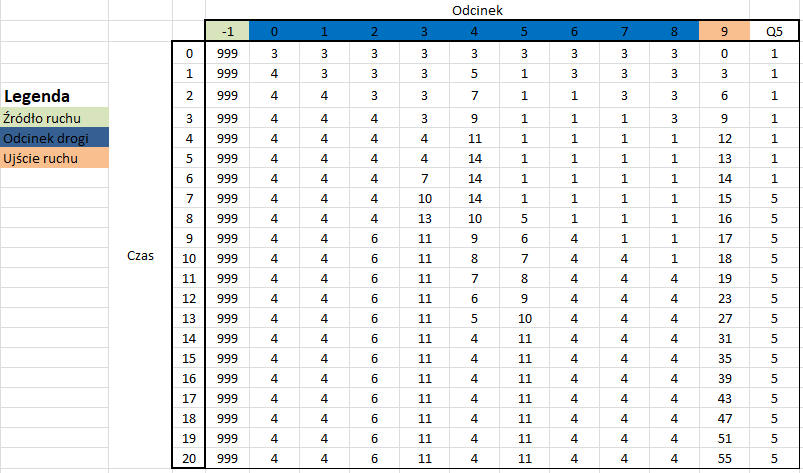
\includegraphics[width=14cm]{images/ctm_przyklad}
	\caption{Tabela ilości pojazdów}
	\label{fig:ctm_przyklad}\end{figure}

\subsection{Przepływ pojazdów na skrzyżowaniu}

\subsubsection{Przykład}

\section{Gottlich dyskretyzacja - to jest bardzo źle}
Początek drogi (k=0)
\[p_0^{t+1}=\frac{1}{4}(3p_0^{t}+p_1^{t})  -\frac{\Delta t}{2 \Delta x}  (f(p_1^t)+f(p^t_0)-2\overline{\gamma}^t) \addtag \]
Centralny odcinek drogi (k=1,...,n-1)
\[p_k^{t+1}=\frac{1}{4}(p_{k-1}^{t}+2p_{k}^{t}+p_{k+1}^t)  -\frac{\Delta t}{2 \Delta x}  (f(p_{k+1}^t)-f(p_{k-1}^t)) \addtag \]
Końcowy odcinek drogi (k=n)
\[p_n^{t+1}=\frac{1}{4}(3p_n^{t}+p_{n-1}^{t})  -\frac{\Delta t}{2 \Delta x}  (2\hat{\gamma}^t -f(p_n^t)-f(p^t_{n-1})) \addtag \]

\[\hat{\gamma}^t_i:=f(p_{0,i}^t)\]
\[\overline{\gamma}^t_i:=f(p_{n,i}^t)\]
Dla dróg $i$ nie będących drogami źródłowymi:
\[\overline{\gamma}^t_i:=\sum_{i \in 
	\delta_{v}^{in}}d_{ij}\hat{\gamma}_{i}(t)\]
Dla dróg źródłowych $\overline{\gamma}^t_i $
jest odgórnie ustalone i ustala jak dużo pojazdów wjeżdża do układu z rozważanej drogi.

STAREEEEEEEEEE

Niech będzie ustalona droga $e$ oraz jej siatka przestrzenna $b_l$. Celem jest przedstawienie wartości gęstości dla odcinków siatki przestrzennej w chwilach $k=0,1,...,K$.
Gęstość w odcinku $b_l$ i czasie $k$ jest zdefiniowana jako:
\[p_{l}^{k}=\int\limits_{{b_{l}}}{\frac{p(x,k)}{\Delta x}dx}. \addtag\]
Na podstawie (\ref{eq:main_diff_eq}) można wywnioskować, że:
\[\int\limits_{b_{l}} {p(x,k+1)- p(x,k)dx} +\int\limits_{k}^{k+1} f(b_{l+1},k)-f(b_{l},k))dk=0 \addtag \label{eq:calki-LWR} \]
Upraszczając otrzymujemy:
\[\Delta x(p_l^{k+1}-p_l^{k}) +\int\limits_{k}^{k+1} f(b_{l+1},k)-f(b_{l},k))dk=0=0 \addtag \]
Wartości gęstości zmieniają się w tylko w chwilach $k$. Wtedy wartości $f(b_{l+1},k)$ i $f(b_l,k)$ są stałe na całym przedziale całkowania $[k,k+1)$. Otrzymujemy równanie:
\[\Delta x(p_l^{k+1}-p_l^{k})  + (f(b_{l+1},k)-f(b_l,k))=0 \addtag \]
Rezultatem jest końcowy rekurencyjny wzór na gęstość ruchu:
\[p_l^{k+1}=p_l^{k}  -\frac{1}{\Delta x}  (f(b_{l+1},k)-f(b_l,k)) \addtag \]







\chapter{Model sieci dróg} \label{chapter:model_sieci_drog}
\section{Wstęp}
Ze względu na dużą złożoność końcowego modelu zostanie przedstawiony najpierw bardzo prosty, podstawowy model. W każdej kolejnej sekcji dodawane będą zmiany przybliżające do ostatecznej postaci. Jest to podejście pozwalające na proste przedstawienie modelu, który zawiera bardzo wiele aspektów m.in:
sygnalizacji świetlnej, wielu dróg, zatoru drogowego, źródła i ujścia ruchu. Zestawienie w jednej sekcji wszystkich tych kwestii byłoby bardzo przytłaczające.

\section{Wektor stanu drogi} \label{sec:wektor_stanu_drogi}
Wektor stanu jest strukturą przedstawiającą stan środowiska. Dla każdego odcinka drogi składuje on wartości zmiennych stanowych. Początkowo zmienną stanu jest identyfikowana jako ilość pojazdów na danym odcinku drogi. 
\subsection{Przykład} \label{subsec:example-single-road}
Niech będzie dana droga z wydzielonymi czterema odcinkami. Przykładowy wektor stanu takiego środowiska to
\[\textbf{x(t)}=\begin{bmatrix}
2 \\ 4 \\ 3 \\ 0
\end{bmatrix} \addtag \]
Zawiera on w sobie następujące informacje dla chwili t:
\begin{itemize}
	\item Są 2 pojazdy na zerowym odcinku
	\item Są 4 pojazdy na pierwszym odcinku
	\item Są 3 pojazdy na drugim odcinku
	\item Nie ma żadnego pojazdu na trzecim odcinku
\end{itemize}

\begin{figure}[H]
	\centering
	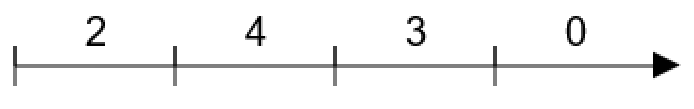
\includegraphics[width=14cm]{images/1_droga_4_odcinki}
	\caption{Droga z ilością pojazdów na poszczególnych odcinkach}
	\label{fig:single_road}
\end{figure}
\section{Rozwój wektora stanu drogi i wprowadzenie macierzy systemu}
Początkowy model przepływu pojazdów zakłada, iż wszystkie pojazdy w chwili t+1 są o jeden odcinek dalej w swojej podróży niż w momencie $t$. Założone jest, iż żadne nowe pojazdy nie pojawiają się w sieci dróg. Ujście pojazdów znajduje się na końcu ostatniego odcinka. Wszystkie pojazdy będące w chwili $t$ na ostatnim odcinku w chwili $t+1$ opuszczają układ. Formalnym wzorem definiującym rozwój wektora stanu jest:
\[\textbf{x(t+1)}=\textbf{Ax(t)} \addtag \label{eq:single_road} \]
Gdzie $\textbf{A}$ jest macierzą systemu. Definiuje ona sposób przepływu pojazdów. $\textbf{A}$ jest rzadką, kwadratową macierzą o wartościach równych 1 jedynie bezpośrednio 1 wiersz pod główną przekątną macierzy. Takie wartości gwarantują przepływ pojazdów o jeden odcinek w jednym interwale czasowym.
\subsection{Przykład}
Dla przykładu przedstawionego w (\ref{subsec:example-single-road}) zostanie przedstawiony rozwój wektora stanu. Niech zatem
\def \xZero {\begin{bmatrix}
	2 \\ 4 \\ 3 \\ 0
	\end{bmatrix}}
\[\textbf{x(0)}=\xZero \addtag \]
Macierzą systemu jest:
\def \A {\begin{bmatrix}
		0 & 0 & 0 & 0 \\
		1 & 0 & 0 & 0 \\
		0 & 1 & 0 & 0 \\
		0 & 0 & 1 & 0 \\
\end{bmatrix}}

\[
\textbf{A}=\A \addtag
\]
Wedle wzoru (\ref{eq:single_road}) wyliczone zostają kolejne wartości wektora stanu.
\def \xI {\begin{bmatrix}
		0 \\ 2 \\ 4 \\ 3
\end{bmatrix}}
\[
\textbf{x(1)}=\textbf{Ax(0)}=\A \xZero = \xI \addtag
\]
\def \xII {\begin{bmatrix}
		0 \\ 0 \\ 2 \\ 4
\end{bmatrix}}
\[
\textbf{x(2)}=\textbf{Ax(1)}=\A \xI = \xII \addtag
\]
\def \xIII {\begin{bmatrix}
		0 \\ 0 \\ 0 \\ 2
\end{bmatrix}}
\[
\textbf{x(3)}=\textbf{Ax(2)}=\A \xII = \xIII \addtag
\]
\def \xIV {\begin{bmatrix}
		0 \\ 0 \\ 0 \\ 0
\end{bmatrix}}
\[
\textbf{x(4)}=\textbf{Ax(3)}=\A \xIII = \xIV \addtag
\]

\section {Wektor stanu sieci dróg}
W rozdziale (\ref{sec:wektor_stanu_drogi}) przedstawiony został wektor stanu dla pojedynczej drogi. W tym rozdziale zostanie sformułowany wektor stanu dla bardziej ogólnego przypadku - sieci dróg. Sposób przedstawienia wartości stanuch jednak jest bardzo podobny. Dla środowiska zawierającego drogi $e_1,...,e_n$ wektor stanu jest utworzony z wartości stanu kolejnych odcinków tych dróg. 

\subsection{Przykład} \label{subsec:wektor_stanu_siec_przyklad}
Niech będzie dana sieć składająca się z trzech dróg. Dla każdej drogi zostaną wydzielone 2 odcinki. W sumie środowisko posiada 6 odcinków. Odcinki są ponumerowane od 0 co przedstawia poniższy rysunek.
	\begin{figure}[H]
	\centering
	
\includegraphics[width=10cm]{images/env_11}
	\label{fig:env_11}
	\caption{Numeracja odcinków środowiska}
\end{figure}

Niech przykładowym wektorem stanu będzie:
\def \xzero {\begin{bmatrix}
		8 \\ 4 \\ 3 \\ 0 \\ 1 \\ 5
\end{bmatrix}}

\[\textbf{x(t)}=\xzero \addtag \]
Zawiera on w sobie informacje dotyczące ilości pojazdów na poszczególnych odcinkach w chwili t. Poniższy obraz przedstawia ilości pojazdów na poszczególnych odcinkach dla stanu zadanego przez wektor $\textbf{x(t)}$
\begin{figure}[H]
	\centering
	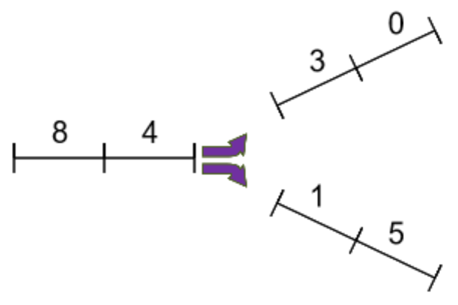
\includegraphics[width=10cm]{images/env_11_843015}
	\caption{Sieć dróg z ilościami pojazdów na poszczególnych odcinkach}
	\label{fig:3_single_road}
\end{figure}

\section{Rozwój wektora stanu sieci dróg}
Przepływ pojazdów niezmiennie jest oparty o założenie, iż w trakcie trwania jednego interwału czasowego pojazdy pokonują 1 odcinek drogi. Nie pojawiają się nowe pojazdy w trakcie trwania symulacji, a ujścia ruchu znajdują się na końcu odcinków 3 i 5.
%Równaniem systemu pozostaje $\textbf{x(t+1)=Ax(t)}$, gdyż do układu nie wpływają nowe pojazdy.\\ \\
Macierz systemu $\textbf{A}$ powinna uwzględnić przepływy pojazdów na skrzyżowaniach. Do tej pory wszystkie pojazdy poruszały się jedynie prosto po odcinkach jednej drogi. W przypadku sieci dróg trzeba uwzględnić przypadek skrzyżowania, gdzie pojazdy mogą obrać różne kierunki ruchu.
%W tym momencie należy przedstawić następującą definicję macierzy $\textbf{A}$:\\
%Wartości macierzy \textbf{A} określają jaka część pojazdów z odcinka zadanego przez indeks kolumny przejeżdża do odcinka zadanego przez indeks wiersza. 
Zdefiniowana zostanie zatem macierz $ \textbf{P} $ prawdopodobieństwa manerwów. Jest to niezmienna w czasie rzadka macierz. Wartości macierzy $ \textbf{P} $ w kolumnie i oraz wierszu j to prawdopodobieństwo przejazdu pojazdu będącego na odcinku i do odcinka j.


\subsection{Przykład}
Rozważone zostanie środowisko (\ref{subsec:wektor_stanu_siec_przyklad}) z dodatkowym założeniem, że 75 procent pojazdów ma zamiar skręcić w prawo. Pozostałe 25 procent wybiera skręt w lewo. 
Srodowisko przedstawiają poniższe obrazki.

\begin{tabular}{| c  | Sc |}
	\hline
	Numeracja odcinków   & Ilości pojazdów \\
	\hline
	\cincludegraphics[width=7cm]{images/env_11}  & \cincludegraphics[width=7cm]{images/env_11_843015_procenty} \\
	\hline 
\end{tabular}
\noindent
Taki sposób przepływu definiuje rzadką macierz prawdopodobieństwa $ \textbf{P} $ o wymiarach 6 na 6.
\begin{itemize}
	\item $\textbf{P}[1,2]=0.25$ wyznacza manewr skrętu w lewo
	\item $\textbf{P}[1,4]=0.75$ wyznacza manewr skrętu w prawo
	\item $\textbf{P}[0,1]=1 \;\; \textbf{P}[2,3]=1 \;\; \textbf{P}[4,5]=1$ co wynika z przepływu pojazdów pomiędzy sekcjami na jednej drodze
	\item Pozostałe wartości macierzy $\textbf{P}$ to zera.
\end{itemize}

\def \P {\begin{bmatrix}
		0 & 0 & 0 & 0 & 0 & 0 \\
		1 & 0 & 0 & 0 & 0 & 0 \\
		0 & 0.25 & 0 & 0 & 0 & 0 \\
		0 & 0 & 1 & 0 & 0 & 0 \\
		0 & 0.75 & 0 & 0 & 0 & 0 \\
		0 & 0 & 0 & 0 & 1 & 0 
\end{bmatrix}}
\[P=\P\]





\def \A{
\begin{bmatrix}
	0 & 0    & 0 & 0 & 0 & 0 \\
	1 & 0    & 0 & 0 & 0 & 0 \\
	0 & 0.25 & 0 & 0 & 0 & 0 \\
	0 & 0    & 1 & 0 & 0 & 0 \\
	0 & 0.75 & 0 & 0 & 0 & 0 \\
	0 & 0    & 0 & 0 & 1 & 0 
\end{bmatrix}
}
\begin{flushleft}
W sytuacji gdy nie ma uwzględnionej sygnalizacji świetlnej oraz pojęcia zatoru macierz systemu jest macierzą prawdopodobieństwa, czyli $A=P$. \linebreak Wartości wektora stanu zmieniają się zgodnie równaniem stanu $\textbf{x(t)}=\textbf{Ax(t-1)}$. Poniżej zapisane są obliczenia.
\end{flushleft}

\def \xI{\begin{bmatrix}
		0 \\ 8 \\ 1 \\ 3 \\ 3 \\ 1
\end{bmatrix}}
\def \xII{\begin{bmatrix}
		0 \\ 0 \\ 2 \\ 1 \\ 6 \\ 3
\end{bmatrix}}
\def \xIII{\begin{bmatrix}
		0 \\ 0 \\ 0 \\ 6 \\ 0 \\ 2
\end{bmatrix}}
\begin{tabular}{| c | c | Sc |}
	\hline
	t   & Równanie stanu & Podgląd środowiska \\
	\hline
	0 & 
	$ \textbf{x(0)} = \xzero$  & \cincludegraphics[width=7cm]{images/env_11_843015_procenty} \\
	\hline 
	1 & $\textbf{x(1)}=\textbf{Ax(0)}=\A \xzero = \xI$  & \cincludegraphics[width=7cm]{images/env_11_081331_procenty} \\
	\hline 
	2 & $\textbf{x(2)}=\textbf{Ax(1)}=\A \xI = \xII$  & \cincludegraphics[width=7cm]{images/env_11_002163_procenty} \\
	\hline 
	3 &	$\textbf{x(3)}=\textbf{Ax(2)}=\A \xII = \xIII$ & \cincludegraphics[width=7cm]{images/env_11_000602_procenty} \\
\hline 
\end{tabular}


\newpage
\section{Wprowadzenie sygnalizacji świetlnej}
Kolejnym etapem rozwoju modelu jest wprowadzenie sygnalizacji świetlnej. Warto zauważyć, że do tej pory rozważane układy były pozbawione jakiegokolwiek sterowania, czego bezpośrednim skutkiem była niezmienność macierzy $\textbf{A}$ w czasie. 
Niech wektor $ [i,j] $ będzie manewrem polegającym na bezpośrednim przejeździe z odcinka $ i $ na odcinek $ j $. Zostanie teraz zdefiniowana macierz sygnalizacji świetlnej $\textbf{S}$. Określa ona wykonalność dowolnego manewru.

\begin{numcases}{S_{ij}=}
1 & dla manewru zezwolonego przez zielone światło \label{eq:allowed_by_light} \\
1 & dla manewru nie wymagającego sygnalizacji świetlnej \label{eq:manewr_existing} \\
0 & dla manewru wstrzymanego przez czerwone światło \label{eq:stopped_by_light} \\
0 & dla niemożliwego manewru \label{eq:manewr_not_existing}
\end{numcases}
Sygnalizacja świetlna zwykle posiada pewną fazę, która określa dozwolone \myref{eq:allowed_by_light} oraz niedozwolone \myref{eq:stopped_by_light} manewry. Fazy świetlne będą oczywiście zmieniane w trakcie symulacji zatem macierz $\textbf{S}$ też jest zmienna w czasie. Wartości macierzy $\textbf{S}$ obejmujące przypadki niemożliwych manewrów \myref{eq:manewr_not_existing} oraz nie wymagających sygnalizacji świetlnej \myref{eq:manewr_existing} są z kolei niezmienne dla ustalonego środowiska.
\subsection{Przykład macierzy sygnalizacji świetlnej} \label{subsec:macierz_sygnalizacji}
Rozważone będzie znane z poprzednich przykładów skrzyżowanie - tym razem mające sygnalizację świetlną z aktywną fazą zezwalającą na manewr [1,2]. Ta sama faza zabrania przejazdu z 1 odcinka do 4. 

\begin{tabular}{| Sc  | Sc |}
	\hline
	Numeracja odcinków   & Ilości pojazdów \\
	\hline
	\cincludegraphics[width=7cm]{images/env_11_faza_0_procenty}  & \cincludegraphics[width=7cm]{images/env_11_lights_0_943015_procenty} \\
	\hline 
\end{tabular}

Poszczególne manewry są następujące:
\begin{itemize}
	\item \myref{eq:allowed_by_light} - Manewrem zezwolonym przez zielone światło  dla fazy $ 0 $ jest $ [1,2] $.
	\item \myref{eq:manewr_existing} - Prawidłowym manewrem bez sygnalizacji świetlnej są manewry $ [0,1] $, $ [2,3] $, $ [4,5] $.
	\item \myref{eq:stopped_by_light} - Dla fazy świetlnej $ 0 $ manewrem zatrzymanym przez czerwone światło  jest $ [1,4] $.
	\item \myref{eq:manewr_not_existing} - Pozostałe manewry są niemożliwe. Przykładem jest $ [0,2] $, gdyż nie ma możliwości bezpośredniego przejazdu z odcinka $ 0 $ do $ 2 $.
\end{itemize}
Macierz sygnalizacji świetlnej dla tego przykładu jest następująca:
\def \S{\begin{bmatrix}
		0 & 0 & 0 & 0 & 0 & 0 \\
		1 & 0 & 0 & 0 & 0 & 0 \\
		0 & 0 & 0 & 0 & 0 & 0 \\
		0 & 0 & 1 & 0 & 0 & 0 \\
		0 & 0 & 0 & 0 & 0 & 0 \\
		0 & 0 & 0 & 0 & 1 & 0 \\
\end{bmatrix}}
\[\textbf{S}=\S\]


\subsection{Macierz systemu uwzględniająca sygnalizację świetlną}
Mając zdefiniowaną zarówno macierz prawdopodobieństwa przejazdów $\textbf{P}$ jak i macierz sygnalizacji świetlnej $ \textbf{S} $ można ustalić macierz systemu $\textbf{A}$ uwzględniającą już sygnalizacje świetlne. Niech $Q$ będzie zbiorem odcinków, które znajdują się bezpośrednio przed ujściem ruchu. Wtedy macierz systemu zdefiniowana jest jako: 
\begin{numcases}{A[i,j]=}
0 & dla $S[i,j]=0 \vee i \in {Q}$ \\
P[i,j] & dla $ S[i,j]=1$ \\
1-\delta(i) & dla $i=j \wedge  i \not\in {Q}$
\end{numcases}
Równanie systemu jest następujące:
\[\textbf{x(t+1)}=\textbf{A(t)x(t)} \addtag \]
Macierz systemu jest teraz zmienna w czasie, zatem w miejse $\textbf{A}$ dotychczasowego równania pojawiło się $\textbf{A(t)}$. \\ \\
\subsection{Przykład rozwoju wektora stanu}
Niech będzie dany układ z przykładu \myref{subsec:macierz_sygnalizacji} z zielonym światłem dla lewoskrętu. W chwili t=2 zostanie zmieniona faza świetlna. Od tego momentu obydwa manewry na skrzyżowaniu są dozwolone.  W chwili t=3 wartości stanu nie są całkowite, co nie jest sprzeczne z modelem matematycznym. Rozwój wektora stanu został przedstawiony w poniższej tabeli.

\def \xzero{\begin{bmatrix}
		9 \\ 4 \\ 3 \\ 0 \\ 1 \\ 5
\end{bmatrix}}
\def \xI{\begin{bmatrix}
		0 \\ 12 \\ 1 \\ 3 \\ 0 \\ 1
\end{bmatrix}}
\def \xII{\begin{bmatrix}
		0 \\ 9 \\ 3 \\ 1 \\ 0 \\ 0
\end{bmatrix}}
\def \xIII{\begin{bmatrix}
		0 \\ 0 \\ 2 \frac{1}{4} \\ 3 \\ 7 \frac{3}{4} \\ 0
\end{bmatrix}}

\def \AZero{
	\begin{bmatrix}
		0 & 0            & 0 & 0 & 0 & 0 \\
		1 & \frac{3}{4}  & 0 & 0 & 0 & 0 \\
		0 & \frac{1}{4}  & 0 & 0 & 0 & 0 \\
		0 & 0            & 1 & 0 & 0 & 0 & \\
		0 & 0            & 0 & 0 & 0 & 0 \\
		0 & 0            & 0 & 0 & 1 & 0 \\
	\end{bmatrix}	
}

\def \AI{
	\begin{bmatrix}
	0 & 0            & 0 & 0 & 0 & 0 \\
	1 & \frac{3}{4}  & 0 & 0 & 0 & 0 \\
	0 & \frac{1}{4}  & 0 & 0 & 0 & 0 \\
	0 & 0            & 1 & 0 & 0 & 0 & \\
	0 & 0            & 0 & 0 & 0 & 0 \\
	0 & 0            & 0 & 0 & 1 & 0 \\
\end{bmatrix}	
}
\def \AII{
	\begin{bmatrix}
	0 & 0            & 0 & 0 & 0 & 0 \\
	1 & 0            & 0 & 0 & 0 & 0 \\
	0 & \frac{1}{4}  & 0 & 0 & 0 & 0 \\
	0 & 0            & 1 & 0 & 0 & 0 & \\
	0 & \frac{3}{4}  & 0 & 0 & 0 & 0 \\
	0 & 0            & 0 & 0 & 1 & 0 \\
\end{bmatrix}
}

\centerline{
\begin{tabular}{| c | c | Sc |}
	\hline
	t   & Równanie stanu & Podgląd środowiska \\
	\hline
	0 &
	$ \textbf{x(0)} = \xzero$  & \cincludegraphics[width=7cm]{images/env_11_lights_0_943015_procenty} \\
	\hline 
	1 & $\textbf{x(1)}=\textbf{A(0)x(0)}=\AZero \xzero = \xI$  & \cincludegraphics[width=7cm]{images/env_11_lights_0_0121301_procenty} \\
	\hline 
	2 & $\textbf{x(2)}=\textbf{A(1)x(1)}=\AI \xI = \xII$  & \cincludegraphics[width=7cm]{images/env_11_lights_01_093100_procenty} \\
	\hline 
	3 &	$\textbf{x(3)}=\textbf{A(2)x(2)}=\AII \xII = \xIII$ & \cincludegraphics[width=7cm]{images/env_11_lights_koncowe_procenty} \\
	\hline 
\end{tabular}
}




\section{Wprowadzenie źródeł ruchu }
Wszystkie poprzednie przykłady układów ruchu drogowego szybko kończyły się stanem w którym nie było już żadnych pojazdów na drogach. W tej sekcji zostanie przedstawiony sposób napływania nowych pojazdów do układu. 
Wprowadzony zostanie wektor źródłą $\textbf{u(t)}$ definiujący pojazdy pojawiające się w układzie. Jest on zmienny w czasie, a jego wartości określają ile pojazdów pojawia się w następnej chwili w poszczególnych odcinkach układu.
Równanie systemu uwzględniające zródła ruchu to:
\[\textbf{x(t)}=\textbf{A(t-1)x(t-1)} + \textbf{u(t-1)} \label{eq:stan_u}   \addtag{}\]
\subsection{Przykład}
Rozważony zostanie prosty przykład, który nie uwzględnia wcześniej wprowadzonych pojęć sygnalizacji świetlnej oraz zatoru. Przedstawione zostanie środowisko składające się z dwóch dróg, które nie są ze sobą w żaden sposób połączony.
\begin{figure}[H]
	\centering
	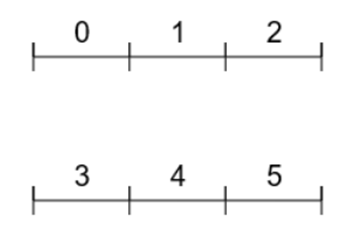
\includegraphics[width=8cm]{images/env_12}
	\label{fig:env_12}
	\caption{Numeracja odcinków środowiska}
\end{figure} \noindent
Pojazdy wzdłóż dróg kończąc swój bieg po przejechaniu przez odcinki 5 i 2 co przedstawia macierz systemu $A$:
\def \A{\begin{bmatrix}
0 & 0 & 0 & 0 & 0 & 0 \\
1 & 0 & 0 & 0 & 0 & 0 \\
0 & 1 & 0 & 0 & 0 & 0 \\
0 & 0 & 0 & 0 & 0 & 0 \\
0 & 0 & 0 & 1 & 0 & 0 \\
0 & 0 & 0 & 0 & 1 & 0
\end{bmatrix}}
\[A=\A \]
Pragnąc by do odcinków 0 i 3  napływało odpowiednio po 4, 8, 20 oraz 3, 7, 5 pojazdów należy zdefiniować ciąg wektorów $\textbf{u(t)}$ w sposób przedstawiony w poniższej tabeli.

\def \xzero{\begin{bmatrix}
		0 \\ 8 \\ 1 \\ 3 \\ 3 \\ 1
\end{bmatrix}}
\def \xI{\begin{bmatrix}
		4 \\ 0 \\ 8 \\ 3 \\ 3 \\ 3
\end{bmatrix}}
\def \xII{\begin{bmatrix}
		8 \\ 4 \\ 0 \\ 7 \\ 3 \\ 3
\end{bmatrix}}
\def \xIII{\begin{bmatrix}
		20 \\ 8 \\ 4 \\ 5 \\ 7 \\ 3
\end{bmatrix}}
\def \uZero{\begin{bmatrix}
		4 \\ 0 \\ 0 \\ 3 \\ 0 \\ 0
\end{bmatrix}}
\def \uI{\begin{bmatrix}
		8 \\ 0 \\ 0 \\ 7 \\ 0 \\ 0
\end{bmatrix}}
\def \uII{\begin{bmatrix}
		20 \\ 0 \\ 0 \\ 5 \\ 0 \\ 0
\end{bmatrix}}

\centerline{
\begin{tabular}{| c | c | Sc | c |}
	\hline
	t   & Równanie stanu & Podgląd środowiska & $ \textbf{u(t)} $ \\
	\hline
	0 & 
	$ \textbf{x(0)} = \xzero$  & \cincludegraphics[width=5cm]{images/env_12_t0} & $\uZero$ \\
	\hline 
	1 & $\textbf{x(1)}=\textbf{Ax(0)}+\textbf{u(0)}=\A \xzero + \uZero = \xI$  & \cincludegraphics[width=5cm]{images/env_12_t1} & $\uI $ \\
	\hline 
	2 & $\textbf{x(2)}=\textbf{Ax(1)}+\textbf{u(1)}=\A \xI + \uI = \xII$  & \cincludegraphics[width=5cm]{images/env_12_t2} & $\uII $ \\
	\hline 
	3 &	$\textbf{x(3)}=\textbf{Ax(2)}+\textbf{u(2)}=\A \xII + \uII = \xIII$ & \cincludegraphics[width=5cm]{images/env_12_t3} & \\
	\hline 
\end{tabular}
}
\section{Zatory drogowe}
Dotychczasowe przedstawienie macierzy systemu $ \textbf{A} $ nie zawiera w sobie jeszcze pojęcia zotoru drogowego. W jednym interwale czasowym moze przejechac przez odcinek astronomiczna wrecz liczba pojazdów. Wprowadzona zostanie zatem funkcja zatoru ograniczająca przejazdy w przypadku zbyt dużej liczby pojazdów. Dziedziną funkcji zatoru $ f $ jest zbiór wszystkich manewrów $ [i,j] $, takich że $ i \neq j $. Funkcja zatoru jest jednak zależna także od wartości stanowych wektora $\textbf{x}$, a przede wszystkim od ilości pojazdów na odcinkach $i$ oraz $j$ czyli $x[i],x[j]$. Wartości funkcji $f$ należą do przedziału $[0,1]$.
Macierz stanowa $\textbf{A}$ z uwzględnieniem zatorów dla układu z $ n $ odcinkami przedstawia się następująco:

\def \Af {\begin{bmatrix}
		1-\delta(0) & f(1,0) & ... & f(n,0) \\
		f(0,1) &1-\delta(1)& ... & f(n,1) \\
		f(0,2) &f(1,2)& ... & f(n,2) \\
		...   &...& ... & ... \\
		f(0,n) &f(1,n)& ... & 1-\delta(n)
\end{bmatrix}}

\[\textbf{A}=\Af \addtag \label{eq_A_z_korkiem} \]
Gdzie $\delta$ to suma wszystkich wartości danej kolumny z wyłączeniem tych na głównej przekątnej. W przypadku odcinków zakończonych ujściem, aby wyzerować wartości $\delta$ przyjmuje wartość 1. Formalnie $\delta$ to:
\begin{numcases}{\delta(i)=}
\sum_{j\in{\{0,...,n\}},j!=i} f(i,j) & dla odcinka $i$ nie zakończonego ujściem \\
1 & dla odcinka $i$ zakończonego ujściem
\end{numcases}

\subsection{Przykład zatoru na pojedynczej drodze} \label{subsec:zator_f10}
Rozważmy poniższe środowisko składające się z drogi posiadającej 4 odcinki.
\begin{figure}[H]
	\centering
	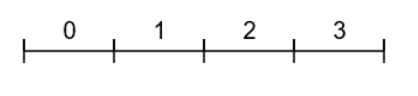
\includegraphics[width=14cm]{images/env_13}
	\caption{Droga z numeracją odcinków}
	\label{fig:env_13}
\end{figure}
Należy skonstruować pewną funkcję zatoru. Niech jej celem będzie, aby przez jeden interwał czasowy maksymalnie 10 pojazdów przejeżdżało przez odcinek drogi. Następująca funkcja gwarantuje takie zachowanie:

\begin{numcases}{f(i,j)=}
\textbf{P}[i,j] & dla $ j=i+1 \wedge x[i]<10$ - przejazd bez zatoru \label{eq:fmanewr_bez_zatoru_fX} \\
\frac{10}{x[i]} & dla $ j=i+1  \wedge x[i] \geq 10$ - przejazd z zatorem \label{eq:fmanewr_zator_fX} \\
0 & dla pozostałych przypadków - niemożliwe manewry \label{eq:fmanewr_not_existing}
\end{numcases} \noindent
 Macierze stanu zostały wyliczone na podstawie wzoru \ref{eq_A_z_korkiem}. W tym przypadku jest to:
\def \A {\begin{bmatrix}
		1-\delta(0) & f(1,0) &   f(2,0) & f(3,0) & \\
		f(0,1) & 1-\delta(1) &   f(2,1) & f(3,1) & \\
		f(0,2) & f(1,2) &   1-\delta(2) & f(3,2) & \\
		f(0,3) & f(1,3) &   f(2,3) & 1-\delta(3) & \\
\end{bmatrix}}
\[A=\A \addtag  \label{eq:A_Idroga_korek}\]

Funkcja $\delta$ dla tego środowiska to:
\begin{numcases}{\delta(i)=}
f(0,1)+f(0,2)+f(0,3) & dla $i = 0 $
\\
f(1,0)+f(1,2)+f(1,3) & dla $i = 1 $
\\
f(2,0)+f(2,1)+f(2,3) & dla $i = 2 $
\\
1 & dla $i = 3 $
\end{numcases}

\def \xzero {\begin{bmatrix}
		17 \\ 2 \\ 11 \\ 4
\end{bmatrix}}

\def \xI {\begin{bmatrix}
		7 \\ 10 \\ 3 \\ 10
\end{bmatrix}}

\def \xII {\begin{bmatrix}
		0 \\ 6 \\ 10 \\ 3
\end{bmatrix}}

\def \Azero {\begin{bmatrix}
		\frac{7}{17} & 0 & 0 & 0  \\
		\frac{10}{17} & 0 & 0 & 0  \\
		0 & 1 & \frac{1}{11} & 0  \\
		0 & 0 & \frac{10}{11} & 0  \\
\end{bmatrix}}

\def \AI {\begin{bmatrix}
		0 & 0 & 0 & 0  \\
		1 & 0 & 0 & 0  \\
		0 & 1 & 0 & 0  \\
		0 & 0 & 1 & 0  \\
\end{bmatrix}}

Rozważmy następujący stan początkowy środowiska:

\centerline{
	\begin{tabular}{| c | c | Sc |}
		\hline
		t   & Równanie stanu & Podgląd środowiska  \\
		\hline
		0 & 
		$ \textbf{x(0)} = \xzero$  & \cincludegraphics[width=5cm]{images/env_13_t_0} \\
		\hline 
	\end{tabular}
}
W celu wyliczenia $\textbf{x(1)}$ należy obliczyć $\textbf{A(0)}$, wedle wzoru \myref{eq:A_Idroga_korek}. Wartości 
zerowej kolumny macierzy $A(0)$ są wyliczane w następującej kolejności:
\begin{itemize}
	\item $ A[0,1]=f(0,1) $ to przypadek manewru z zatorem \myref{eq:fmanewr_zator_fX}. Zatem $f(0,1)=\frac{10}{17}$, gdyż $x[0]=17$
	\item $A[0,2]=f(0,2) = 0  \; f(0,3)=0$ to przypadki niemożliwych manewrów \myref{eq:fmanewr_not_existing}.
	\item $A[0,0]=1-\delta(0)=1-f(0,1)-f(0,2)-f(0,3)=1-\frac{10}{17}-0-0=\frac{7}{17}$ pozostaje na odcinku 0.
\end{itemize}
Analogiczne operacje zostają przeprowadzone dla kolejnych kolumn co daje rezultat w postaci:
\[A(0)=\Azero\]
Dalszy rozwój wektora stanu jest przedstawiony w tabeli poniżej.

\centerline{
	\begin{tabular}{| c | c | Sc |}
		\hline
		t   & Równanie stanu & Podgląd środowiska  \\
		\hline
		0 & 
		$ \textbf{x(0)} = \xzero$  & \cincludegraphics[width=5cm]{images/env_13_t_0} \\
		\hline 
		1 & $ \textbf{x(1)} = \textbf{A(0)x(0)} =  \Azero \xzero = \xI$ & \cincludegraphics[width=5cm]{images/env_13_t_1} \\
		\hline 
		2 & $ \textbf{x(2)} = \textbf{A(1)x(1)} = \AI \xI = \xII$ & \cincludegraphics[width=5cm]{images/env_13_t_2} \\
		\hline 
	\end{tabular}
}


\subsection{Przykład zatoru na skrzyżowaniu}
Niech funkcją zatoru będzie funkcja przedstawiona w (\ref{eq:fmanewr_bez_zatoru_fX}-\ref{eq:fmanewr_not_existing})
Rozważmy poniższą sytuację na drogach w chwili $t=0$:
\begin{figure}[H]
	\centering
	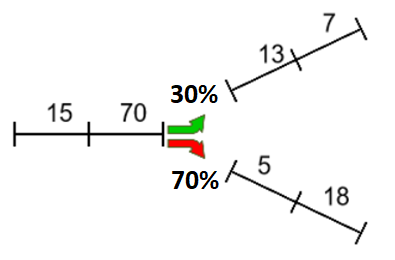
\includegraphics[width=10cm]{images/env_11_1570137518_procenty.png}
	\label{fig:env_11_case_0}
\end{figure}\noindent
\begin{itemize}
	\item Zatory są na odcinkach 0,1,2 i 5 (odpowiednio ilości pojazdów to 15,70,13,18). 
	\item Obecna faza świetlna to 0.
\end{itemize}
Najistotniejszym punktem macierzy sygnalizacji świetlnej jest $ S[1,2]=1 $, co odpowiada zielonemu światłu dla lewoskrętu. Cała macierz $ \textbf{S} $ to:
\def \ScaseZero {\begin{bmatrix}
		1 & 0 & 0 & 0 & 0 & 0 \\
		1 & 1 & 0 & 0 & 0 & 0 \\
		0 & {1} & 1 & 0 & 0 & 0 \\
		0 & 0 & 1 & 1 & 0 & 0 \\
		0 & 0 & 0 & 0 & 1 & 0 \\
		0 & 0 & 0 & 0 & 1 & 1 
\end{bmatrix}}
\def \AcaseZero {\begin{bmatrix}
		\frac{5}{15}  & 0             & 0             & 0 & 0 & 0 \\
		\frac{10}{15} & \frac{60}{70} & 0             & 0 & 0 & 0 \\
		0          	  & \frac{10}{70} & \frac{3}{13}  & 0 & 0 & 0 \\
		0             & 0             & \frac{10}{13} & 0 & 0 & 0 \\
		0             & 0             & 0             & 0 & 0 & 0 \\
		0             & 0             & 0             & 0 & 1 & 0 
\end{bmatrix}}

\[\textbf{S}= \begin{bmatrix}
1 & 0 & 0 & 0 & 0 & 0 \\
1 & 1 & 0 & 0 & 0 & 0 \\
0 & \mathbf{1} & 1 & 0 & 0 & 0 \\
0 & 0 & 1 & 1 & 0 & 0 \\
0 & 0 & 0 & 0 & 1 & 0 \\
0 & 0 & 0 & 0 & 1 & 1 
\end{bmatrix} \addtag \]
Macierz systemu to zatem:
\[\textbf{A}= \begin{bmatrix}
\frac{5}{15}  & 0             & 0             & 0 & 0 & 0 \\
\frac{10}{15} & \frac{60}{70} & 0             & 0 & 0 & 0 \\
0          	  & \mathbf{\frac{10}{70}} & \frac{3}{13}  & 0 & 0 & 0 \\
0             & 0             & \frac{10}{13} & 0 & 0 & 0 \\
0             & 0             & 0             & 0 & 0 & 0 \\
0             & 0             & 0             & 0 & 1 & 0 
\end{bmatrix} \addtag \]
\def \utMinusI{\begin{bmatrix} 
		7 \\ 0 \\ 0 \\ 0 \\ 0 \\ 0 
\end{bmatrix}}
\def \xtMinusI{\begin{bmatrix} 
		15 \\ 70 \\ 13 \\ 7 \\ 5 \\ 18	
\end{bmatrix}}
\def \xt{\begin{bmatrix} 
		12 \\ 70 \\ 13 \\ 10 \\ 0 \\ 5	
\end{bmatrix}}\noindent
Dla przykładu szczegółowo zostaną policzone wartości zerowej kolumny macierzy $\textbf{A}$, która dotyczy pojazdów wyjeżdżających z odcinka 0. Pozostałe wartości są liczone analogicznie.
\begin{itemize}
	\item Korzystając ze wzoru \ref{eq:manewr_zator_f10} ustalone zostaje $f(0,1)=\frac{10}{15}$. Jest to przypadek zatoru i jedynie 10 pojazdów z 15 przemieszcza się do następnego odcinka.
	\item Wartości $f(0,2),(0,3),(0,4),(0,5)$ są równe $0$, gdyż są to przypadki \ref{eq:manewr_not_existing} nieistniejących manewrów.
	\item $A[0,0]=1-\delta(0)=1-f(0,1)-f(0,2)-f(0,3)-f(0,4)-f(0,5)=1- \frac{10}{15} -0-0-0-0= \frac{5}{15}$
\end{itemize}
Stan w momencie $t=1$ wyliczony z równania stanu jest następujący:
\[\textbf{x[1]}=\textbf{A[0]x[0]}=\AcaseZero \cdot \xtMinusI = \xt \]
Poniższy obraz przedstawia sytuację w środowisku w chwili t-1 oraz przepływ pojazdów, który miał miejsce między momentem $t-1$ a $t$.
\begin{figure}[H]
	\centering
	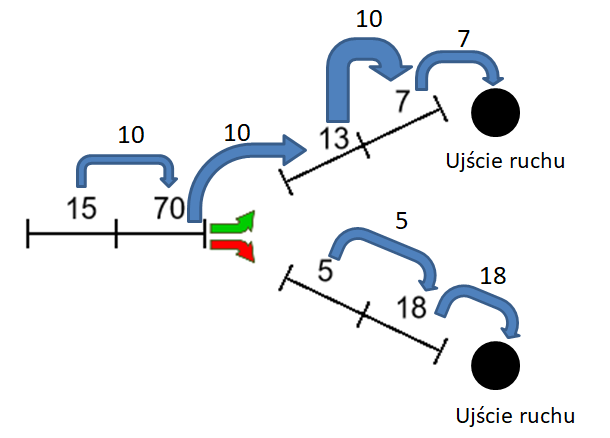
\includegraphics[width=10cm]{images/env_11_przeplyw_korek}
	\label{fig:env_11_case_0_przeplyw}
\end{figure}\noindent
W rezultacie w chwili t obecny jest następujący stan:
\begin{figure}[H]
	\centering
	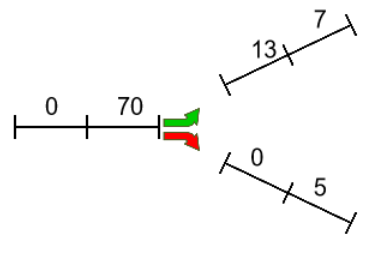
\includegraphics[width=10cm]{images/env_11_po_korku}
	\label{fig:env_11_case_0_po_przeplywie}
\end{figure}\noindent


\chapter {Środowiska symulacyjne i ich nauka}
W tym rozdziale przedstawione zostaną środowiska symulacyjne. Głównym ich elementem jest sieć dróg. Podstawowe informacje na temat działania modelu sieci dróg i ruchu obowiązującego na nich zostały przedstawione w rozdziale \ref{chapter:model_sieci_drog}. Każde środowisko posiada dokładną specyfikacje możliwych faz świetlnych. Do każdego ze skrzyżowań jest przyporządkowany agent, który ma za zadanie podejmować akcje prowadzące do dobrej przepustowości ruchu. Dokładnie zostaną przedstawione przestrzenie decyzyjne i bezpośrednie konsekwencje każdej z akcji. Każde środowisko będzie posiadało swój problem optymalizacyjny i przedstawiony zostanie sposób uczenia, który prowadzi do rozwiązania tego problemu. 
\section{Srodowisko 1}
%(11 na froncie)
Elementy sieci dróg pierwszego środowiska były niejednokrotnie przedstawiane w rozdziale \myref{chapter:model_sieci_drog}, jednak dopiero teraz nastąpi przedstawienie pierwszego pełnego środowiska symulacyjnego. Na model sieci składają się 3 drogi - każda ma po 2 odcinki. Jest jedno skrzyżowanie na którym 75 procent pojazdów skręca w prawo, a pozostałe obierają kierunek w lewo.
\begin{figure}[H]
	\centering
	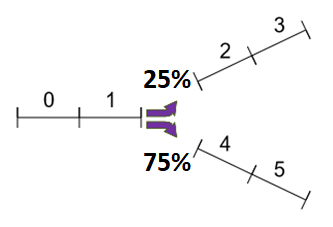
\includegraphics[width=10cm]{images/env_11_procenty}
	\label{fig:env_11}
	\caption{środowisko 11}
\end{figure}

\subsection{Sygnalizacje świetlne}	
\begin{figure}[H]
	\centering
	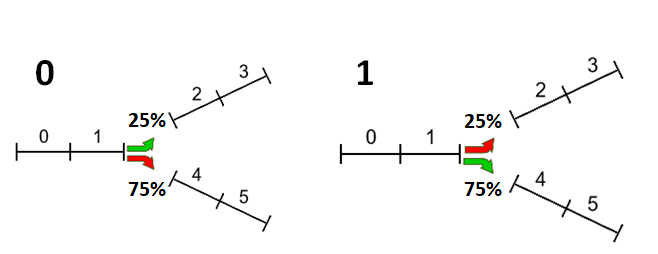
\includegraphics[width=17cm]{images/env_11_fazy_procenty_no_yellow}
	\label{fig:env_11_fazy}
	\caption{środowisko 11 - fazy świateł}
\end{figure}\noindent
Skrzyżowanie posiada 2 fazy świetlne przedstawione powyżej. Faza 0 umożliwia skręt w lewo (manewr [1,2]) z kolei faza 1 umożliwia skręt w prawo (manewr [1,4]).

\subsection{Przestrzeń decyzyjna}
Agent ma dwie możliwe akcje do podjęcia - 0 oraz 1. Obydwie powodują aktywacje odpowiadającej im fazy świetlnej.

\subsection{Zatory drogowe}
Wykorzystana w modelu zostanie funkcja zatoru przedstawiona w rozdziale \myref{subsec:zator_f10}, czyli:

\begin{numcases}{f(i,j)=}
\textbf{P}[i,j] & dla $ j=i+1 \wedge x[i]<10$ - przejazd bez zatoru \label{eq:manewr_bez_zatoru_f10} \\
\frac{10}{x[i]} & dla $ j=i+1  \wedge x[i] \geq 10$ - przejazd z zatorem \label{eq:manewr_zator_f10} \\
0 & dla pozostałych przypadków - manewr [i,j]
\end{numcases} \noindent

\subsection{Uczenie}
\subsubsection*{Ogólny zarys}
W trakcie symulacji treningowych do drogi wjeżdża 9 pojazdów w czasie jednego interwału. Po jednej iteracji algorytmu uczenia następuje symulacja w pełni zachłanna.
\subsubsection*{Cel nauki}
Celem nauki jest uzyskanie jak największej liczby pojazdów, które opuszczą rozwidlenie dróg.
\subsubsection*{Pożądane zachowanie}
Pożądanym zachowaniem jest utrzymywanie fazy 1. Jest ona w każdym przypadku lepsza lub równa fazie 0. Spowodowane jest to tym, że więcej pojazdów skręca w prawo. W przypadku gdy przed rozwidleniem drogi jest conajmniej 40 pojazdów poprawną akcją jest także wybór fazy 0. Nie powinno jednak dojść do aż takiego zatoru.
\subsubsection*{Sygnał wejściowy}
Sygnał wejściowy to ilości pojazdów przed skrzyżowaniem.
\subsubsection*{Przykład sygnału wejściowego}
Sygnał wejściowy $ \textbf{x}=[4,7] $ zawiera w sobie informację, iż na odcinku zerowym są 4 pojazdy oraz na pierwszym - jest ich 7. 
\subsubsection*{Sposób uczenia}
Zastosowana została metoda uczenia przedstawiona w \myref{learning:DQN_single_agent}. Następujące stałe określające model uczenia to:
\begin{itemize}
	\item $\gamma = 0.9$ - stopa dyskontowa
	\item $\alpha = 0.01$ - stała szybkości uczenia (ang. learning rate)
	\item Generowanych jest jednorazowo 50 epizodów. Każdy ma 200 interwałów czasowych.
	\item Wygenerowane zbiory danych są dzielone w proporcjach 80 i 20 procent dla odpowiednio treningu i walidacji.
	\item Warunkiem stopu jest 60 sekund działania algorytmu.
	\item Sieć neuronowa posiada 1 ukrytą warstwę z 10 neuronami.
	\item Za uczenie odpowiada sieć neuronowa biblioteki Keras. Posiada ukrytą warstwę z 10 neuronami i funkcją aktywacji relu. Optymalizacja jest przeprowadzana przez metodę Adam z funkcją straty błędu średniokwadratowego i parametrem $learning\_rate = 0,01$. 
	\item Epizod zachłanny trwa 200 interwałów czasowych.
\end{itemize}

\subsubsection{Wyniki uczenia}
Za każdym razem już po trzeciej iteracji algorytmu osiągane jest pożądane zachowanie agenta. Dla każdego stanu agent wybiera akcję 1. Nie tworzą się zatory i wszystkie pojazdy opuszczają układ (oczywiście z wyjątkiem tych, które pojawiły się w dwóch ostatnich interwałach czasowych).

\section{Srodowisko 2}
%(14 na froncie)
Na model sieci składają się 3 drogi - każda ma po 2 odcinki. Istnieje jedno skrzyżowanie z dwiema drogami wlotowymi i jedną wylotową.
	\begin{figure}[H]
	\centering
	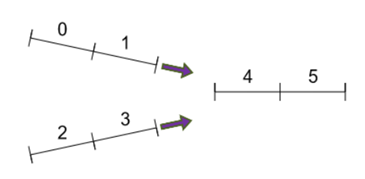
\includegraphics[width=10cm]{images/env_14}
	\label{fig:env_14}
	\caption{środowisko 2}
\end{figure}

\subsection{Sygnalizacje świetlne}	
\begin{figure}[H]
	\centering
	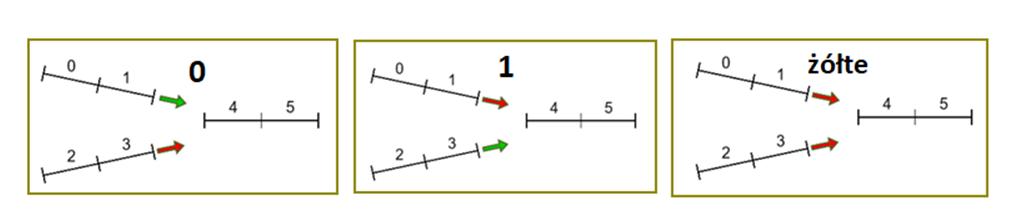
\includegraphics[width=17cm]{images/env_14_fazy}
	\label{fig:env_14_fazy}
	\caption{środowisko 2 - fazy świateł}
\end{figure}\noindent
Skrzyżowanie posiada 3 fazy świetlne przedstawione powyżej. Faza 0 umożliwia przejazd przez skrzyżowanie z górnej drogi (manewr [1,4]) z kolei faza 1 umożliwia wjazd z drogi dolnej (manewr [3,4]). Faza "żółte" blokuje przejazd przez skrzyżowanie.

\subsection{Przestrzeń decyzyjna}
Przestrzeń decyzyjną oraz konsekwencje akcji podjętych przez agenta przedstawia poniższa tabela:
\begin{figure}[H]
	\centering
	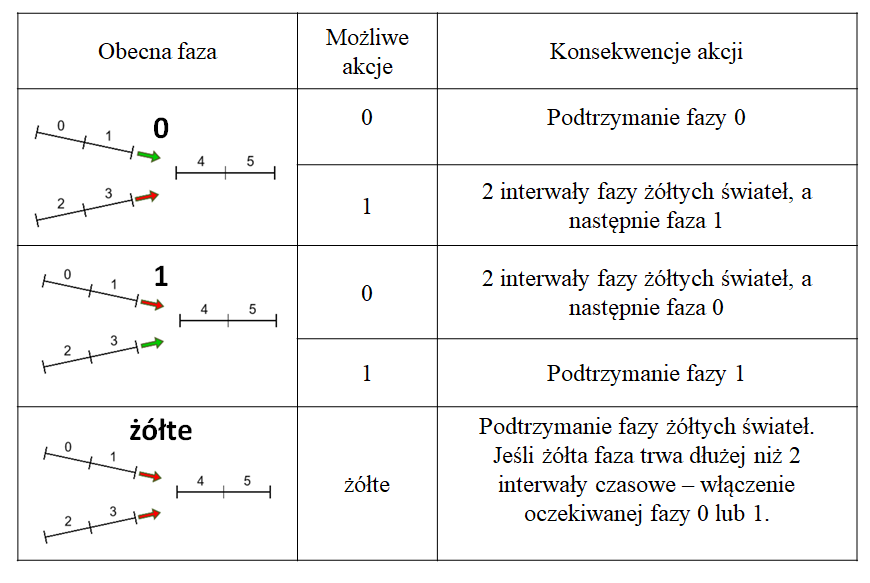
\includegraphics[width=17cm]{images/env_14_akcje}
	\label{fig:env_14_akcje}
\end{figure} \noindent

\subsection{Zatory drogowe}
Wykorzystana w modelu zostanie funkcja zatoru przedstawiona w rozdziale \myref{subsec:zator_f10}, czyli:

\begin{numcases}{f(i,j)=}
\textbf{P}[i,j] & dla $ j=i+1 \wedge x[i]<10$ - przejazd bez zatoru \label{eq:manewr_bez_zatoru_f10} \\
\frac{10}{x[i]} & dla $ j=i+1  \wedge x[i] \geq 10$ - przejazd z zatorem \label{eq:manewr_zator_f10} \\
0 & dla pozostałych przypadków - manewr [i,j]
\end{numcases} \noindent
Zezwala ona na jednoczesny wjazd maksymalnie 10 pojazdów na dowolny odcinek drogi.
\subsection{Uczenie}
\subsubsection{Ogólny zarys}
Początkowo do każdej z dróg wjeżdżają po 2 pojazdy w jednym interwale czasowym. Na koniec każdej iteracji nauki przeprowadzane są symulacje w pełni zachłanne. Agent ma za zadanie wykonywać akcje, które w trakcie symulacji pozwolą na opuszczenie skrzyżowania przez conajmniej 98 procent pojazdów. W przypadku spełnienia tego warunku następuje zwiększenie ilości wjeżdżających do układu pojazdów. Ten proces jest powtarzany, aż do momentu gdy przez 10 iteracji uczenia nie uzyskany zostanie warunek 98 procent pojazdów opuszczających skrzyżowanie. Moment stopu spodziewany jest na chwilę, gdy na każdą z dróg będzie wjeżdżało około 5 pojazdów. Nie ma możliwości, by przejeżdżało więcej niż 10 pojazdów, a tyle właśnie pojawia się w układzie. Muszą zatem wtedy pojawiać się zatory.

\subsubsection{Cel nauki}
Bezpośrednim celem nauki jest uzyskanie jak największej ilości pojazdów wjeżdżających do sieci. Aby to się stało agenci muszą podejmować decyzje, które pozwalają na opuszczenie sieci jak największej ilości pojazdów. 
\subsubsection{Spodziewany wynik}
Moment stopu spodziewany jest na chwilę, gdy na każdą z dróg będzie wjeżdżało około 5 pojazdów (w sumie 10 pojazdów). Zgodnie z opisem modelu ruchu - maksymalnie 10 pojazdów może przejechać w jednej chwili przez skrzyżowanie, zatem muszą się tworzyć zatory przy większej ilości pojazdów.
\subsubsection{Pożądane zachowanie agenta}
Pożądane zachowanie agenta w tym przypadku nie jest jednoznaczne do określenia. Z pewnością jeśli na drodze na której jest zielone światło jest conajmniej 10 pojazdów, to warto podtrzymać fazę świetlną. Zmiana sygnalizacji powoduje 2 interwały karencji, podczas których żaden pojazd nie przejedzie i może to być czynnikiem decydującym o pozostaniu przy obecnej fazie. Jaka powinna być akcja w przypadku gdy zielone światło jest dla drogi z mniejszą niż 10 ilością pojazdów? Wtedy agent powinien odnaleźć złoty środek i jeśli na drugiej drodze jest dużo pojazdów - może zmienić światło. 
\subsubsection*{Sygnał wejściowy}
Wektor stanu posiada 4 wartości. Pierwsze dwie z nich to ilości pojazdów przed skrzyżowaniem. Kolejne określają aktualną fazę świetlną.
\subsubsection*{Przykłady sygnałów wejściowych}
\begin{itemize}
	\item Sygnał wejściowy $ \textbf{x}=[8,2,0,1] $ zawiera w sobie informację, iż na odcinku zerowym jest 8 pojazdów oraz na pierwszym - jest ich 2. Aktywna jest faza 1.
		\item Sygnał wejściowy $ \textbf{x}=[7,5,1,0] $ zawiera w sobie informację, iż na odcinku zerowym jest 7 pojazdów oraz na pierwszym - jest ich 5. Aktywna jest faza 0.
\end{itemize}
\subsubsection{Sposób uczenia}
Zastosowana została metoda uczenia przedstawiona w \myref{learning:DQN_single_agent}. 

Następujące stałe oraz ustalenia określają szczegóły uczenia:
\begin{itemize}
	\item $\gamma = 0.9$ - stopa dyskontowa
	\item Parametr $\epsilon$ jest początkowo równy 1 (w pełni losowe epizody). Z każdą iteracją jest zmniejszany o 0,01 aż do wartości $\epsilon=0,2$.
	\item Generowanych jest jednorazowo 10 epizodów. Każdy z nich trwa 1000 interwałów czasowych.
	\item Wygenerowane zbiory danych są dzielone w proporcjach 80 i 20 procent dla odpowiednio treningu i walidacji.
	\item Za uczenie odpowiada sieć neuronowa biblioteki Keras. Posiada ona 3 ukryte warstwy (10,14,10 neuronów) z funkcjami aktywacji relu. Optymalizacja jest przeprowadzana przez metodę Adam z funkcją straty błędu średniokwadratowego i parametrem $learning\_rate = 0,01$. 
\end{itemize}

\subsubsection*{Wyniki uczenia}
Algorytm szybko uzyskuje kolejne warunki 98 procent pojazdów przejeżdżających przez skrzyżowanie. Dopiero przy 4,97 wjeżdzających pojazdach na drogę widoczny jest zastój, który powoduje warunek stopu.
Najlepszy wynik to średnio 9,48 pojazdów przejeżdżających w jednej chwili przez skrzyżowanie. Jest to dobry wynik zważając na to, iż potencjalnie najwyższy możliwy wynik do osiągnięcia jest w granicy 9,94. Z 9940 pojazdów 450 nie opuściło skrzyżowania. Zatem przy niemalże 5 pojazdach napływających do układu powstają korki, co jest naturalnym zjawiskiem - wynikającym z ograniczeń ruchu, a nie nieoptymalnej sygnalizacji świetlnej.

\section{Srodowisko 3}
%(16 na froncie)
\begin{figure}[H]
	\centering
	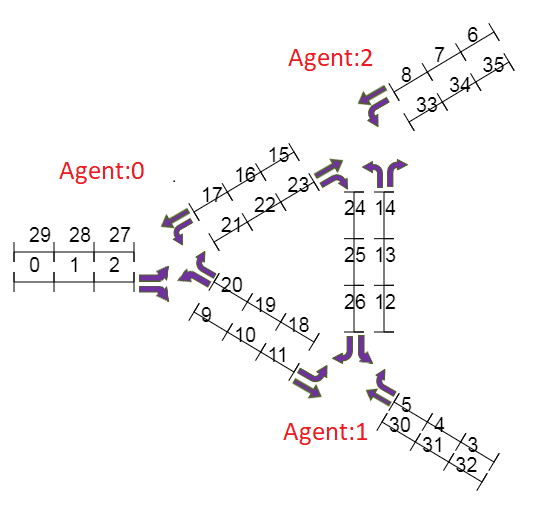
\includegraphics[width=10cm]{env_4_agenci}
	\label{fig:env_4_agenci}
	\caption{środowisko 4}
\end{figure}

Środowisko posiada 12 jednokierunkowych dróg. Każda droga ma 3 odcinki co daje w sumie 36 odcinków (są numerowane od 0 co widać na rysunku \ref{fig:env_4_agenci}).
W sieci dróg znajdują się 3 skrzyżowania. Do każdego z nich jest przypisany agent, który odpowiada za sterowanie sygnalizacją świetlną.
\subsection{Sygnalizacje świetlne}
Każde skrzyżowanie posiada 4 fazy świetlne przedstawione poniżej. Fazy 0,1 i 2 są fazami, które posiadają pewne zielone światła. Zmiana pomiędzy tymi fazami nie jest natychmiastowa i następuje dopiero po 2 interwałach fazy żółtych świateł.
\begin{figure}[H]
	\centering
	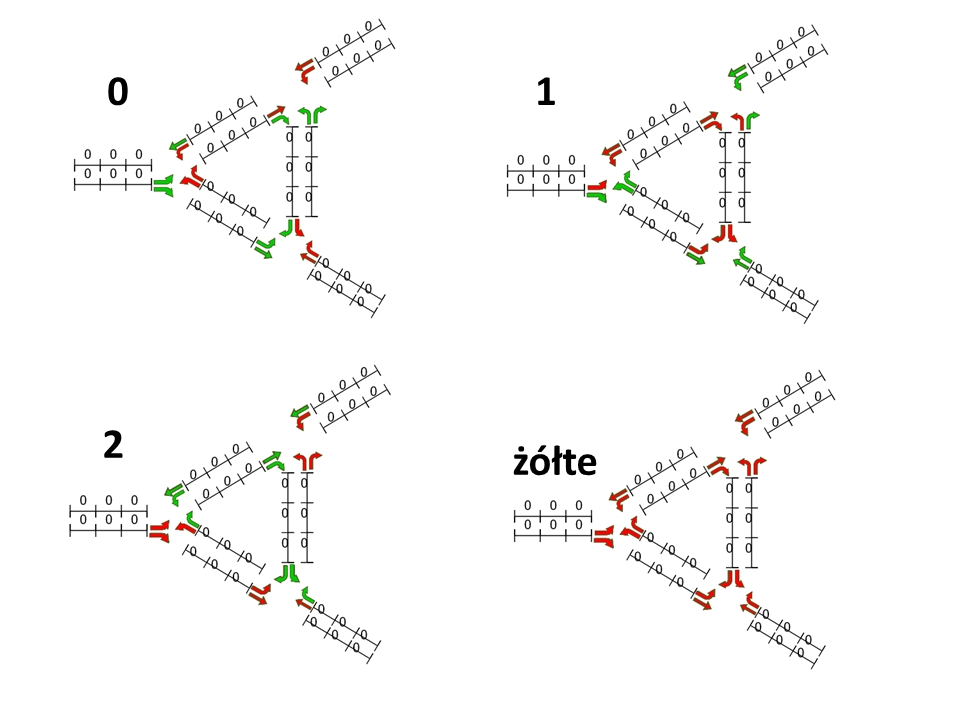
\includegraphics[width=14cm]{env_4_fazy}
	\label{fig:env_4_fazy}
	\caption{środowisko 4 - fazy świateł}
\end{figure}
\subsection{Przestrzeń decyzyjna} \label{subsec_pn_dec}
Przedstawiona zostanie przestrzeń decyzyjna jedynie dla agenta 0, jednak dla pozostałych dwóch przestrzenie decyzyjne są analogiczne. Schemat zmiany faz jest identyczny, jedynie manewry danych faz są inne.
\begin{figure}[H]
	\centering
	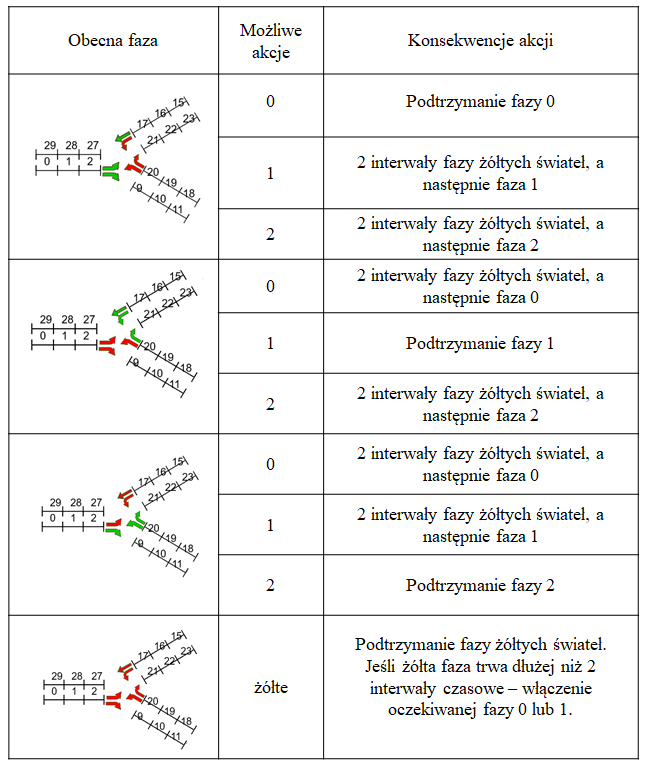
\includegraphics[width=14cm]{images/env_14_akcje_agent0_tabela}
	\label{fig:env_4_akcje_agent_0}
	\caption{środowisko 4 - fazy świateł}
\end{figure}
\subsection{Zatory drogowe}
Wykorzystana w modelu zostanie funkcja zatoru przedstawiona w rozdziale \myref{subsec:zator_f10}, czyli:
\begin{numcases}{f(i,j)=}
\textbf{P}[i,j] & dla $ j=i+1 \wedge x[i]<10$ - przejazd bez zatoru \label{eq:manewr_bez_zatoru_f10} \\
\frac{10}{x[i]} & dla $ j=i+1  \wedge x[i] \geq 10$ - przejazd z zatorem \label{eq:manewr_zator_f10} \\
0 & dla pozostałych przypadków - manewr [i,j]
\end{numcases} \noindent
Zezwala ona na jednoczesny wjazd 10 pojazdów na dowolny odcinek drogi.
\subsection{Uczenie}
\subsubsection*{Sygnał wejściowy}
Sieć neuronowa przypisana do każdego z agentów przyjmuje jako sygnał wejściowy 6 elementową tablicę. Pierwsze 3 elementy to ilości pojazdów na odcinkach będących przed skrzyżowaniem przypisanym do agenta. Pozostałe 3 elementy mają wartości z zakresu $\{0,1\}$. Określają one aktualną fazę świetlną. 
\subsubsection*{Przykład sygnału wejściowego}
Sygnał wejściowy $x=[5,17,2,0,0,1]$ przedstawia informację, iż przed skrzyżowaniem są kolejki odpowiednio 5,17 i 2 pojazdów. Ostatnie 3 elementy oznaczają, że aktualna faza świetlna to 2.

\subsection*{Uczenie}
\subsubsection{Ogólny zarys}
Początkowo do każdej z dróg wjeżdża po jednym pojeździe. Na koniec każdej iteracji nauki przeprowadzane są symulacje w pełni zachłanne. Agent ma za zadanie wybierać akcje, które pozwolą na opuszczenie sieci dróg przez conajmniej 95 procent pojazdów. Jeśli ten warunek zostanie spełniony następuje zwiększenie ilości wjeżdżających pojazdów o 20 procent dotychczasowej wartości. W przypadku gdy ten warunek nie zostanie spełniony przez 15 kolejnych symulacji następuje koniec nauki. 
\subsubsection*{Cel nauki i spodziewany wynik}
Bezpośrednim celem nauki jest uzyskanie jak największej ilości pojazdów wjeżdżających do sieci. Aby to się stało agenci muszą podejmować decyzje, które pozwalają na opuszczenie sieci jak największej ilości pojazdów. Moment stopu spodziewany jest na chwilę, gdy na każdą z dróg będzie wjeżdżało niecałe 10 pojazdów. Zgodnie z opisem modelu ruchu - maksymalnie 10 pojazdów może wjechać w jednej chwili na dany odcinek, zatem muszą się tworzyć zatory przy większej ilości pojazdów.

\subsubsection*{Sposób uczenia}
Zastosowana została metoda uczenia przedstawiona w \myref{learning:DQN_single_agent}. 

Następujące stałe oraz ustalenia określają szczegóły uczenia:
\begin{itemize}
	\item $\gamma = 0.9$ - stopa dyskontowa
	\item Parametr zachłanności $\epsilon$ jest początkowo równy 1 (w pełni losowe epizody). Z każdą iteracją jest zmniejszany o 0,01 aż do wartości $\epsilon=0,2$.
	\item Generowanych jest jednorazowo 20 epizodów. Każdy z nich trwa 300 interwałów czasowych.
	\item Wygenerowane zbiory danych są dzielone w proporcjach 80 i 20 procent dla odpowiednio treningu i walidacji.
	\item Za uczenie odpowiada sieć neuronowa biblioteki Keras. Posiada ona 3 ukryte warstwy (10,14,10 neuronów) z funkcjami aktywacji relu. Optymalizacja jest przeprowadzana przez metodę Adam z funkcją straty błędu średniokwadratowego i parametrem $learning\_rate = 0,01$. 
	\item Epizod zachłanny trwa 1000 interwałów czasowych.
\end{itemize}
\subsubsection{Wyniki uczenia}
Moment stopu jest osiągnięty przy 8.9 pojazdów napływających do sieci ruchu. Najwyższy osiągnięty wyniki 20 epizodów z takim napływem ruchu to 90 procent. Żadna z akcji nie jest zaniechana - agenci conajmniej kilkadziesiąt razy podejmują każdą z dostępnych akcji w zachłannym epizodzie.

\section{Srodowisko 4 - kampus B Politechniki Łódzkiej}
\begin{figure}[H]
	\centering
	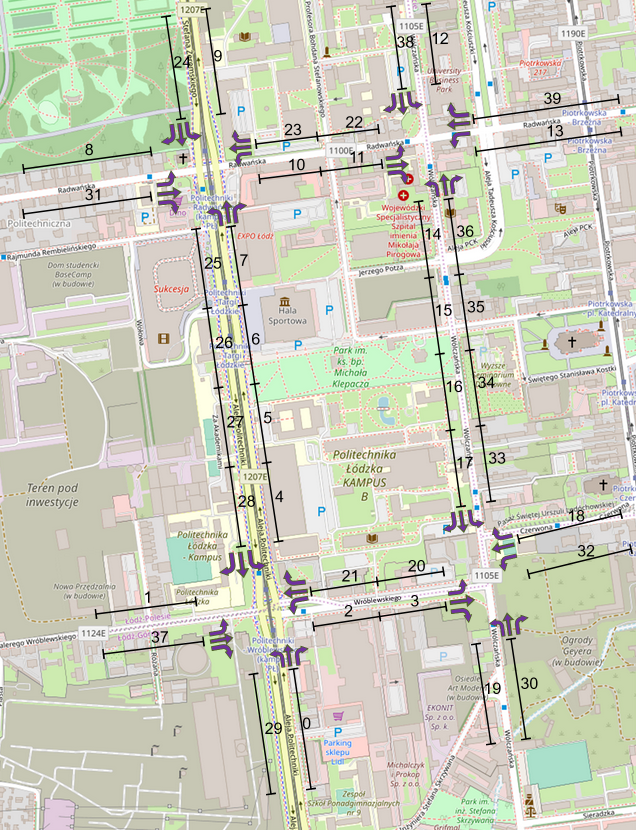
\includegraphics[width=10cm]{images/env_poli}
	\label{fig:env_poli}
	\centering
	\caption{Środowisko 5 - Skrzyżowania wokół kampusu B Politechniki Łódzkiej. Mapy Open Street Map}
\end{figure}
Struktura środowiska bazuje na rzeczywistej sieci dróg znajdującej się w Łodzi. Sieć wyznaczają ulice Wróblewskiego, Wólczańska, Radwańska i aleja Politechniki Łódzkiej. Środowisko posiada 40 odcinków w tym 4 odcinki źródłowe (0,8,30,39) i 4 odcinki wylotowe (1,8,13,19). Drogi krzyżują się w 4 miejscach. Na dowolnym skrzyżowaniu kierowcy mogą wykonać manewry skrętu w lewo, w prawo oraz jazdy prosto. 


\subsection{Sygnalizacje świetlne}
Każde skrzyżowanie posiada 5 faz świetlnych. Fazy 0,1,2 i 3 są fazami, które posiadają pewne zielone światła. Zmiana pomiędzy tymi fazami nie jest natychmiastowa i następuje dopiero po 2 interwałach fazy żółtych świateł. Skrzyżowanie ulic Wróblewskiego, Wólczańskiej i Czerwonej posiada inne od pozostałych trzech skrzyżowań fazy świetlne. Wynika to z kolizyjności lewoskrętów z ulic Wróblewskiego i Czerwonej. Poniższa tabela przedstawia możliwe fazy świetlne.

\begin{tabular}{| Sc  | Sc | Sc|}
	\hline
	Faza   & \specialcell{Wólczańska/\\Wróblewskiego/\\Czerwona} & Pozostałe 3 skrzyżowania \\
	\hline
	0  & 
	\cincludegraphics[height=4cm]{images/env_poli_faza_0_wol} & 	\cincludegraphics[height=4cm]{images/env_poli_faza_0_pozostale} \\
	\hline 
	1  & 
	\cincludegraphics[height=4cm]{images/env_poli_faza_1_wol} & 	\cincludegraphics[height=4cm]{images/env_poli_faza_1_pozostale} \\
	\hline 
	2  & 
	\cincludegraphics[height=4cm]{images/env_poli_faza_2_wol} & 	\cincludegraphics[height=4cm]{images/env_poli_faza_2_pozostale} \\
	\hline 
	3  & 
	\cincludegraphics[height=4cm]{images/env_poli_faza_3_wol} & 	\cincludegraphics[height=4cm]{images/env_poli_faza_3_pozostale} \\
	\hline 
	Żółte  & 
	\cincludegraphics[height=4cm]{images/env_poli_faza_zolte_wol} & 	\cincludegraphics[height=4cm]{images/env_poli_faza_zolte_pozostale} \\
	\hline 
\end{tabular}

\subsection{Przestrzeń decyzyjna}
Analogicznie do poprzednich przestrzeni decyzyjnych z fazą żółtych świateł - przykładowo \myref{subsec_pn_dec}.
\subsection{Zatory drogowe}
Wykorzystana w modelu zostanie funkcja zatoru przedstawiona w rozdziale \myref{subsec:zator_f10}, czyli:
\begin{numcases}{f(i,j)=}
\textbf{P}[i,j] & dla $ j=i+1 \wedge x[i]<10$ - przejazd bez zatoru \label{eq:manewr_bez_zatoru_f10} \\
\frac{10}{x[i]} & dla $ j=i+1  \wedge x[i] \geq 10$ - przejazd z zatorem \label{eq:manewr_zator_f10} \\
0 & dla pozostałych przypadków - manewr [i,j]
\end{numcases} \noindent
Zezwala ona na jednoczesny wjazd maksymalnie 10 pojazdów na dowolny odcinek drogi.
\subsection{Uczenie}
\subsubsection*{Ogólny zarys}
Do każdej z dróg źródłowych wjeżdża pewna ilość pojazdów co interwał. Początkowo ilość ta jest zadana przez zmienną losową o rozkłądzie lognormalnym o parametrach $\delta=1, \mu=1$. Na koniec każdej iteracji nauki przeprowadzane są symulacje w pełni zachłanne. Agent ma za zadanie wykonywać akcje, które w trakcie symulacji pozwolą na opuszczenie skrzyżowania przez conajmniej 95 procent pojazdów. W przypadku spełnienia tego warunku następuje zwiększenie parametru $\mu$ o 20 procent dotychczasowej wartości. Konsekwencją zwiększenia $\mu$ jest większa ilość wjeżdżających do układu pojazdów. Ten proces jest powtarzany, aż do momentu gdy przez 15 kolejnych iteracji uczenia nie uzyskany zostanie warunek 95 procent pojazdów opuszczających skrzyżowanie.
\subsubsection*{Cel nauki}
Bezpośrednim celem nauki jest uzyskanie jak największej wartości parametru $\mu$. Aby to się stało agenci muszą podejmować decyzje, które pozwalają na opuszczenie sieci możliwie jak największej ilości pojazdów.
\subsubsection*{Wyniki uczenia}
Moment stopu przypadł na $\mu=7,43$ pojazdu wjeżdżającego na drogę. Okazuje się, że proces uczenia doprowadził do zaniechania przez agentów manewrów lewoskrętów (akcje 0 i 1). Jest to z pewnością niepożądane zachowanie, jednak można było się go spodziewać, gdyż nagrody zostały wymodelowane tak, by gratyfikować jedynie przepływ - nieistotne z jakiego manewru. 
\subsection{Modyfikacja środowiska}
Zostaje nałożona dodatkowa restrykcja związana z przestrzenią akcji. Spośród 100 kolejno podjętych akcji powinna znaleźć się każda możlwa akcja.
\subsubsection*{Wyniki uczenia zmodyfikowanego środowiska}
Wyniki uczenia są identyczne do wariantu bez restrykcji wystąpienia wszystkich faz. Wyeliminowany został jednak niepożądany efekt zaniechania lewosrkętów.

\chapter{Przegląd metod optymalizacyjnych}
\section{Kategorie uczenia maszynowego}
Uczenie maszynowe to dziedzina wchodząca w skład nauk zajmujących się sztuczną inteligencją. Samo uczenie w najprostszym kształcie może być rozumiane jako dobór parametrów na podstawie dostępnych danych. Uczenie maszynowe jest powszechnie dzielone na 3 kategorie nauki \cite{machineLearningClassification}.
\begin{enumerate}
	\item \textbf{Nadzorowane} \\
	Dane używane do uczenia nazywane są zbiorem treningowym. Każdy pojedynczy element zbioru treningowego ma informacje wejściowe oraz pewną pożądaną wartość wyjściową. W trakcie uczenia algorytm dopasowuje swoje parametry tak aby na podstawie danych wejściowych mógł przewidzieć wartość wyjściową. Przykładami uczenia nadzorowanego jest np. rozpoznawanie tekstu pisanego, detekcja obiektów na zdjęciach.
	\item \textbf{Nienadzorowane}
	Uczenie nienadzorowane różni się od nadzorowanego tym, że nie  są znane pożądane wartości wyjściowe. Celem nauki jest na podstawie podobieństw poszczególnych elementów zgrupowanie ich do odpowiednich klas. Przykładem uczenia nienadzorowanego może być np. klasyfikacja gatunków drzew na podstawie danych o ich wysokościach i szerokości korony drzew.
	\item \textbf{Wzmocnione}
	W środowisku uczenia ze wzmocnieniem istnieje agent, który jest odpowiedzialny za podejmowanie pewnych decyzji. Każda decyzja ma wpływ na stan środowiska, które zwraca agentowi nagrodę. Celem uczenia ze wzmocnieniem jest ustalenie strategii maksymalizującej skumulowaną wartość nagród.
\end{enumerate}
Ze wszystkich trzech kategorii uczenie ze wzmocnieniem odpowiada problemowi rozważanym w rozdziale Y. Szczegółowy opis uczenia ze wzmocnieniem zostanie przedstawiony w następnej sekcji.
\section{Uczenie ze wzmocnieniem}
Schemat uczenia ze wzmocnieniem składa się z następujących elementów:
\begin{enumerate}
	\item \textbf{Agent} jest odpowiedzialny za podejmowanie pewnych decyzji. Ma on wiedzę na temat obecnego stanu środowiska i otrzymuje w każdym kroku czasowym sygnał nagrody. Jego decyzje niebezpośrednio wpływają na stan środowiska.
	\item \textbf{Środowisko} jest przestrzenią posiadającą dynamiczny stan widoczny dla agenta. Chociaż to agent podejmuje akcje, to środowisko ma zdefiniowany model zmiany stanu. Model zmiany stanu może być stochastyczny oraz niewidoczny dla agenta. Oznacza to, że dwie te same akcje podjęte w tym samym stanie nie zawsze przyniosą identyczny następny stan. Innymi słowy agent nie może być stuprocentowo pewny rezultatów swoich akcji. Środowiska rozważane w rozdziale x są jednak w pełni deterministyczne. Środowisko jest także nadawcą sygnału nagrody.
	\item \textbf{Strategia} definiuje sposób doboru akcji przez agenta w danej chwili. Jest to funkcja, która przyjmuje stan środowiska i zwraca akcje, która powinna być przeprowadzona. 
	\item \textbf{Sygnał nagrody} definiuje cel problemu uczenia ze wzmocnieniem. W każdym kroku czasowym środowisko wysyła agentowi liczbę rzeczywistą, która jest nazywana nagrodą(reward). Wartości nagród są czynnikiem wpływającym na zmianę strategii, gdyż zadaniem agenta jest maksymalizacja nagród. Wartość nagród zatem definiuje, które zdarzenia są dobre, a które złe dla agenta. Biologicznym odpowiednikiem dodatniej nagrody jest przyjemność, a ujemnej - ból \cite{berridge2000reward}. 
	\item \textbf{Funkcja wartości} zwraca wartość stanu czyli oczekiwaną sumę nagród jakie agent osiągnie w przyszłości będąc aktualnie w tym stanie. 
\end{enumerate}
\begin{figure}[H]
	\centering
	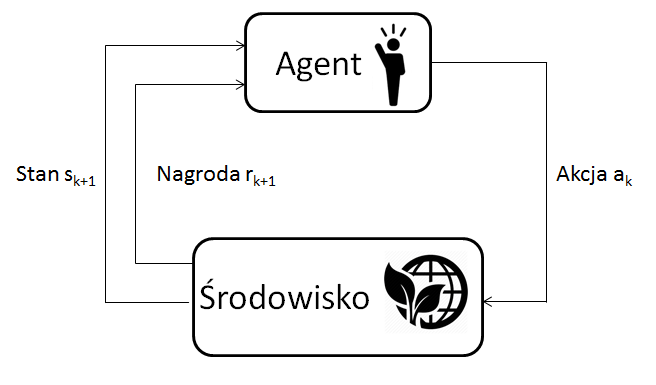
\includegraphics[width=14cm]{agent-srodowisko}
	\caption{Interakcje pomiędzy agentem a środowiskiem.}
	\label{fig:agent-srodowisko}
\end{figure}
\newpage
Algorytmy uczenia ze wzmocnieniem zazwyczaj stosuje się do rozwiązywania problemu procesu decyzyjnego Markowa. Sam \textbf{proces decyzyjny Markowa} jest zdefiniowany jako uporządkowana czwórka $(S,A,P_a,R_a)$, gdzie:
\begin{enumerate}
	\item $S$ to zbiór stanów
	\item $A$ to zbiór akcji. Notacją $A_s$ oznaczane są możliwe akcje dla stanu $s$.
	\item $P_a(s,s')=Pr(s_{t+1}=s'|s_t=s,a_t=a)$ to prawdopodobieństwo, że akcja $a$ wykonana w stanie $s$ w chwili $t$ doprowadzi do stanu $s'$ w chwili $t+1$.
	\item $R_a(s,s')$ to oczekiwana nagroda otrzymana w wyniku akcji podjętej w stanie $s$ prowadzącej do stanu $s'$.
\end{enumerate}

Problemem procesu decyzyjnego Markowa jest odnalezienie optymalnej strategii. Strategia określona jest jako funkcja $\pi(s)$ przyjmująca jako argument stan, a zwracająca podejmowaną akcję. Celem optymalizacji jest odnalezienie strategii maksymalizującej wartość:
\[
G=\sum_{k=0}^{K} \gamma^k R_{k} \addtag \label{eq:Markov_maximize}
\]
Chociaż we wzorze \myref{eq:Markov_maximize} nie ma strategii $\pi(s)$, to wpływa ona na otrzymywane nagrody $R_{k}$ w każdej chwili $k$.\\
$\gamma \in (0,1]$ jest czynnikiem dyskontującym. Idea dyskontowania nagród zaczerpnięta jest z rachunku finansowego. Przykładowo wpływ na konto kapitału 1000 złotych po upływie roku czasu jest z pewnością bardziej wartościowy niż za 20 lat. Pieniądze w matematyce finansowej są prawie zawsze liczone w czasie i tak samo należy postępować z nagrodami. Im wartość $\gamma$ jest bliższa 0 tym bardziej istotne są początkowe nagrody. Dla $\gamma=1$ wszystkie nagrody są równie istotne - bez względu na czas ich otrzymania.\\
Analogicznie do (\ref{eq:Markov_maximize}) jest ustalona funkcja wartości stanu. Jako wartość stanu $s$ określone jest:
\[
G_t=\sum_{k=t}^{K} \gamma^k R_{k}=R_{t}+\gamma R_{t+1}+\gamma^{2} R_{t+2}+...+\gamma^{K}R_K \addtag \label{eq:Markov_state_value_G}
\]
Zostanie przedstawiony teraz przykład obliczeniowy. Agent podejmuje decyzje na których podstawie otrzymuje ciąg  nagród $R_0=0, R_1=2,R_2=6,R_3=-1,R_4=2,R_5=1$. Czynnik dyskontujący $\gamma$ jest równy 0,9. Jaka jest wartość $G$ oraz $G_1,G_2,G_3,G_4,G_5$?\\
\begin{figure}[H]
	\centering
	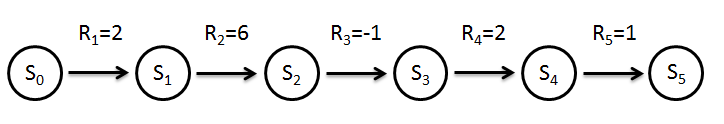
\includegraphics[width=14cm]{rewards-graph}
	\caption{Ciąg nagród i stanów.}
	\label{fig:agent-srodowisko}
\end{figure}\noindent
Najłatwiej obliczenia rozpocząć od $G_5$ i skończyć na $G_1$.
\[G_5=R_5.  \addtag\]
Dla pozostałych t:
\[G_{t}=R_{t}+\gamma G_{t+1} \label{eq:G_reccurential}. \addtag \]\\
$G_5=R_5=1.$\\
$G_4=R_4+\gamma G_{5}=\;\;2+0,9\cdot 1=2,9.$\\
$G_3=R_3+\gamma G_{4}=\!-1+0,9\cdot2.9=1,61.$\\
$G_2=R_2+\gamma G_{3}=\;\;6+0,9\cdot1,61 \approx 7,45.$\\
$G_1=R_1+\gamma G_{2}=\;\;2+0,9\cdot 7,45 \approx 8,70.$\\
$G\;\,=R_0+\gamma G_{1}=\;\;0+0,9\cdot 8,70 \approx 7,83.$\\

\section{Metoda Monte Carlo On-Policy}
Metody Monte Carlo są szeroką klasą algorytmów, których wyniki oparte są o losowe próbkowanie. Nie potrzebują one żadnej wiedzy na temat środowiska - akceptowalne są zarówno środowiska deterministyczne jak i stochastyczne. Algorytmy Monte Carlo uczenia ze wzmocnieniem są dzielone na dwie kategorie - On-Policy oraz Off-policy. W pracy zostanie przedstawiona metoda on-policy, która różni się od off-policy jedynie sposobem doboru momentu eksploracji. Metoda on-policy zakłada, iż ustalana jest pewna liczba $\epsilon$ bliska zeru. Określa ona prawdopodobieństwo kroku eksploracji, czyli wyboru losowej akcji. Pozostałe akcje są wybierane w sposób zachłanny, czyli podejmowana jest najbardziej wartościowa dostępna akcja. Algorytm przedstawiony jest poniższym pseudokodem.
\begin{enumerate}
	\item Zainicjuj słowniki:
	\begin{enumerate}
		\item $Q(s,a)$ - Wartość określa opłacalność wyboru akcji a w stanie s
		\item $Returns(s,a)$ - Wartość słownika to tablica wartości $G$ wyliczonych na podstawie wzoru (\ref{eq:Markov_state_value_G}).
		\item $\pi(s)$ - Określa jaka akcja ma zostać podjęta dla stanu s. Początkowo wszystkie akcje są wybrane losowo.
	\end{enumerate}
	\item Zasymuluj pełny epizod wedle strategii $\pi$
	\item Zoptymalizuj strategię $\pi$ - dla każdej pary (s,a) - stanu i akcji, które pojawiły się w epizodzie
	\begin{enumerate}
		\item Wylicz $G$ rekurencyjnie wedle wzoru (\ref{eq:G_reccurential}) t.j. $G_{t}=R_{t}+\gamma G_{t+1}$.aa
		\item Do tablicy Returns(s,a) dodaj wartość $G$
		\item $Q(s,a)=avg(Returns(s,a))$
		\item $\pi(s)=a^*$. Gdzie $a^*$ to taka akcja, że $Q(s,a^*)\geq Q(s,a)$ dla każdego $a 
		\in A$. Jeśli został jednak wylosowany krok ekspolarcji, wtedy $\pi(s)$ jest losowo wybraną akcją $a \in A$.
	\end{enumerate}
\end{enumerate}
\subsubsection{Uwagi}
Rozsądnym jest iterowanie w kroku 3a) w kolejności odwrotnej do chronologicznej, gdyż ułatwia wykorzystanie wzoru (\ref{eq:G_reccurential})
\\ Warto zauważyć następujące zalety metody Monte Carlo:
\begin{enumerate}
	\item Brak potrzeby wiedzy na tematu modelu środowiska - t.j. rozkładu prawdopodobieństwa konsekwencji akcji.
	\item Nie wymaga często nierealnego założenia, iż stan środowiska może zostać sztywno ustalony przez programistę. Wymagana jest jedynie możliwość przeprowadznia pełnych epizodów, co jest nieporównywalnie słabszym założeniem.
	\item Adekwatne dane - czasu treningowy jest poświęcony dla stanów, które są często odwiedzane. Z kolei te, które nie pojawiają się prawie wcale - nie marnują dużo czasu w procesie nauki.
\end{enumerate}
Jak się okazało dla bardziej złożonych środowisk (3 i 4 dodaj refa) - z dużą przestrzanią stanu i akcji powyższy algorytm jest niewystarczający. Należy zauważyć, że bardzo podobne stany nie mają ze sobą w tym algorytmie żadnej korelacji. Gdy przestrzeń jest bardzo duża, ograniczenia czasowe mogą nie pozwolić na eksplorację każdego stanu. Jako przykład problemu niech stanem środowiska będzie kolejka przed skrzyżowaniem. Wtedy dwa bardzo podobne stany $[3,22,72]$ oraz $[3,22,73]$ są od siebie różne i symulacje muszą prześledzić każdy z tych stanów. Zakładając, że wartości każdej zmiennej są ze zbioru $\{0,1,...,100\}$ liczność przestrzeni stanu jest równa aż 1 000 000. Lepiej skalującym rozwiązaniem jest zastosowanie sieci neuronowych zamiast tablic. Zostanie ono przedstawione w następnej sekcji.

\section{Metoda Monte Carlo On-Policy z użyciem sieci neuronowej} \label{learning:DQN_single_agent}
Podstawową różnicą względem algorytmu Monte Carlo opartego na tablicach jest inny wzór rozwoju wartości. Formuła jest następująca:
\[Q(s,a) \leftarrow (1-\alpha)Q(s,a) + \alpha [r + \gamma \max_{a' \in A'} Q(s',a')] \addtag \label{eq:Q_DQN} \]
\begin{itemize}
	\item $ s,a $ to para stanu i akcji, które pojawiły się w trakcie symulacji
	\item $\alpha$ to stała szybkości uczenia (ang. learning rate)
	\item $ r $ to nagroda przydzielona podczas symulacji dla akcji $ a $ podjętej w stanie $ s $
	\item $\gamma \in [0,1]$  to stopa dyskontowa
	\item $ s' $ to stan do którego doprowadziła akcja $ a $ podjęta w stanie $ s $ podczas symulacji
	\item $ A' $ to przestrzeń możliwych akcji do podjęcia w stanie $ s' $
\end{itemize}
Nie jest ten wzór jednak używany do składowania wartości Q w tablicach, a do generowania danych do sieci neuronowej. Całkowity algorytm jest następujący:
\begin{enumerate}
	\item Dla każdego agenta utwórz sieć neuronową. Będzie ona na wejście przyjmować stany środowiska. Wyjściowym sygnałem jest opłacalność akcji możliwych do podjęcia w stanie danym na wejściu - czyli Q.
	\item Zasymuluj pewną ilość epizodów wedle losowej strategii. Akcje są wybierane w $\epsilon$ - greedy sposób. Zapisuj dane wygenerowane podczas tych epizodów: \label{symulacja_50}
	\begin{enumerate}
		\item Stany środowiska
		\item Podjęte akcje
		\item Przydzielone nagrody
	\end{enumerate}
\item Na podstawie zapisanych danych utwórz następujące zbiory wykorzystane w sieci neuronowej:
\begin{enumerate}
\item Zbiór sygnałów wejściowych (x-batch). Pojedynczym elementem tego zbioru jest tablica przedstawiająca stan środowiska.
\item Zbiór oczekiwanych sygnałów wyjściowych (y-batch), czyli opłacalności akcji do podjęcia w stanie zadanym na wejścu.
Dla elementu odpowiadającego akcji, która została podjęta w symulacji wylicz wartość wedle równania \myref{eq:Q_DQN}. Dla elementów odpowiadających pozostałym akcją, które nie zostały podjęte - sieć neuronowa przewiduje nagrodę. 
\end{enumerate}
\item Podziel powyższe zbiory na segment treningowy i walidacyjny.
\item Trenuj sieć neuronową do momentu, gdy wyniki dla zbioru walidacyjnego się polepszają.
\item Jeśli spełniony jest warunek stopu - przerwij algorytm. W przeciwnym razie przejdź do \ref{symulacja_50}.

\subsection{Wariant z fazą żółtych świateł}
W momencie fazy żółtych świateł agent podejmuje zawsze akcję "żółte". Nie potrzebne jest zatem wyliczanie wartości Q dla tej wymuszonej akcji. Aby nie obligować sieci neuronowej do aproksymacji nieistotnych wartości zostaną podjęte następujące kroki.
Jeśli dana jest wiedza na temat długości fazy żółtych świateł należy zastąpić wzór \myref{eq:Q_DQN} poniższymi formułami. Niech faza żółtych świateł trwa $k$ interwałów czasowych, wted: \\
dla akcji a utrzymania obecnej fazy:
\[Q(s,a) \leftarrow (1-\alpha)Q(s,a) + \alpha [r + \gamma \max_{a' \in A'} Q(s',a')], \addtag \label{eq:Q_DQN_I} \]
dla akcji a zmiany obecnej fazy:
\[Q(s,a) \leftarrow  (1-\alpha)Q(s,a) + \alpha [\gamma^{k} r + \gamma^{k+1} \max_{a' \in A'} Q(s',a')]. \addtag \label{eq:Q_DQN_II} \]

\end{enumerate}


\bibliographystyle{plain}

\bibliography{refs}
\end{document}
